\documentclass[pre,twocolumn,twoside,superscriptaddress,floatfix, aps, 10pt]{revtex4-1}

\usepackage{currfile}
\lefthyphenmin=3
\righthyphenmin=2

\usepackage{graphicx,epsfig,verbatim,enumerate}
\usepackage{amssymb,amsmath}
\usepackage{ifthen}

% Fonts and typesetting settings
\usepackage[sc]{mathpazo}
\usepackage[T1]{fontenc}
\linespread{1.05} % Palatino needs more space between lines
\usepackage{microtype}
\usepackage{textcomp}

\usepackage{longtable}

\usepackage{mathtools}

\newboolean{twocolswitch}

\newcommand{\www}[1]{\url{#1}}
\newcommand{\req}[1]{(\ref{#1})}
\newcommand{\Req}[1]{Eq.~(\ref{#1})}

% Lettrines
\usepackage{lettrine}

%useful shortcuts
\def\R{\ensuremath{\mathbb{R}}} %\ensuremath adds math mode, if forgotten
\def\Q{\ensuremath{\mathbb{Q}}}
\def\N{\ensuremath{\mathbb{N}}}
\def\Z{\ensuremath{\mathbb{Z}}}
\def\C{\ensuremath{\mathbb{C}}}

%shorcuts with arguments
\newcommand{\abs}[1]{\left\vert#1\right\vert} %nice absolute values
\newcommand{\bt}[1]{\textbf{#1}} %bold
\newcommand{\eq}[1]{\begin{align*}#1\end{align*}} %aligned equations
\newcommand{\norm}[1]{\left\lVert#1\right\rVert} %vector norm
\renewcommand{\eq}[1]{\begin{align*}#1\end{align*}} %aligned equations

%piecewise function

%\begin{displaymath}
%   f(x) = \left\{
%     \begin{array}{lr}
%       1 & : x \in \mathbb{Q}\\
%       0 & : x \notin \mathbb{Q}
%     \end{array}
%   \right.
%\end{displaymath} 


%environment
\newcommand{\tab}{\phantom{ssss}}


\usepackage{color}
\newcommand{\todo}[1]{\noindent\textcolor{blue}{{$\Box$ #1}}}

%colors
\definecolor{javagreen}{rgb}{0.25,0.5,0.35} %dark green color
\definecolor{lightblue}{rgb}{0.149,0.545,0.824} %solarized blue
\definecolor{sred}{rgb}{0.863, 0.196, 0.184} %solarized red

\newcommand{\blue}[1]{{\leavevmode\color{lightblue}{#1}}} %solarized blue 
\newcommand{\green}[1]{{\leavevmode\color{javagreen}{#1}}} %command for green
\newcommand{\red}[1]{{\leavevmode\color{sred}{#1}}} %solarized red
\newcommand{\gray}[1]{{\leavevmode\color[gray]{0.5}{#1}}} %gray text
\newcommand{\Prob}[1]{{\rm Pr}\left(#1\right)}


\setboolean{twocolswitch}{true}


\begin{document}

\title{\protect
A Web of Human Knowledge: 
Unravelling Wikipedia's First Link Network
}

\author{
\firstname{Mark}
\surname{Ibrahim}
}
\email{mark.s.ibrahim@uvm.edu}

\affiliation{Department of Mathematics \& Statistics, 
    Computational Story Lab,  \\
    The University of Vermont, Burlington, VT 05401.}

\author{
\firstname{Christopher}
\surname{M. Danforth}
}
\email{chris.danforth@uvm.edu}

\affiliation{Department of Mathematics \& Statistics, 
    Computational Story Lab,  \\
    The University of Vermont, Burlington, VT 05401.}


\author{
\firstname{Peter}
\surname{Sheridan Dodds}
}

\email{peter.dodds@uvm.edu}

\affiliation{Department of Mathematics \& Statistics, 
    Computational Story Lab,  \\
    The University of Vermont, Burlington, VT 05401.}

\begin{abstract}
  \protect
Apples, oranges, and the most obscure Dylan song too---is everything a few clicks from Philosophy? 
Within Wikipedia, the surprising answer is yes: nearly all 
paths lead to Philosophy.
Wikipedia is the largest, most meticulously indexed collection of human knowledge ever amassed. 
More than information about a topic though, Wikipedia is a marvelous web of naturally emerging relationships.  
By following the First Link in an article, we connect entries to form a directed network within Wikipedia: Wikipedia's First Link Network. 
Here we study the English edition of Wikipedia's First Link Network for insight into how we relate topics, ideas, people, objects, and events.  


We algorithmically parse all 4.7 million articles to construct a map of Wikipedia's First Link Network. 
In a novel approach to uncover structure, we traverse every possible path through the network, 
measuring the accumulation of First Links, path lengths, basins, cycles, and even particular articles funneling links into the cycles.
We discover many scale-free distributions, find Philosophy at a salient center, and uncover a flow from specific to general with 
basins around fundamental notions such as Community, State, and Science. 
Curiously, we also observe a gravitation towards topical articles including Health Care and Fossil Fuel.
These findings enrich our view of how we connect and structure
an ever growing load of information.
 
\end{abstract}

\maketitle

\section{Introduction}



Wikipedia is a towering achievement of the modern era. 
At no point in history has a larger or more meticulously indexed collection of human knowledge 
existed.
Wikipedia contains 37 million articles in 283 languages, 
with coverage spanning everything from little known ancient battles to the latest pharmaceutical drugs 
\cite{stats} \cite{drugs}.
All this information does not lie dormant. 
Wikipedia is the sixth most visited
site in the world, surpassing 18 billion page views in a single month
\cite{wiki_views}.
The most widely used general reference, Wikipedia has amassed an awe-inspiring collection of human knowledge.

It's not surprising then to see Wikipedia as the object of many studies. 
Researchers have examined the cultural dynamics among editors,
\cite{editors}
the accuracy of the content relative to traditional encyclopedias,
\cite{accuracy1}
\cite{accuracy2}
the disciplines and topics covered 
\cite{coverage}
and bias against portions of the population
\cite{bias_women}.
Wikipedia's content has also proven a powerful tool. 
Researchers have used Wikipedia to identify missing dictionary entries
\cite{missing_entries},
cluster short text
\cite{clustering},
compute semantic relatedness
\cite{semantic_relatedness},
and disambiguate meaning \cite{disambiguating}.

While these many studies have dissected and fruitfully applied Wikipedia's content,
few have examined the connections among the many articles.
Beyond information, Wikipedia is a web 
relating ideas. 
Within the body text of Wikipedia articles hyperlinks reference
other Wikipedia articles.
A hyperlink from one Wikipedia article to another is a way to relate the ideas
conveyed in the two articles 
\cite{relevance}.
The notion that hyperlinks convey information about the content of a
page has proved successful in numerous domains from search engine algorithms 
such as PageRank 
\cite{pagerank} 
to topic classification
\cite{classifier}.
We treat a hyperlink as a mechanism to connect two ideas. 

The authors of a Wikipedia article choose where and whether to include a 
hyperlink reference to another Wikipedia article.
Authors must include hyperlinks in the article's markup.
In describing a particular topic, each set of authors decides which articles are the most
relevant references.
For example, the hyperlinks in the "Train" article depend only on what its authors 
decide are pertinent articles to reference.
The collection of hyperlinks emerges from the independent choice of each article's authors. 
The first hyperlink to another Wikipedia article marks the earliest moment in the body text where the authors
choose to connect the information discussed to that of another article.
By following the first hyperlink to another article in the English edition of
Wikipedia, we connect the ideas in one article to those in another, ultimately forming a directed network: 
{\it Wikipedia's First Link Network} (FLN).

\begin{figure*}[tp!]
  \centering	
  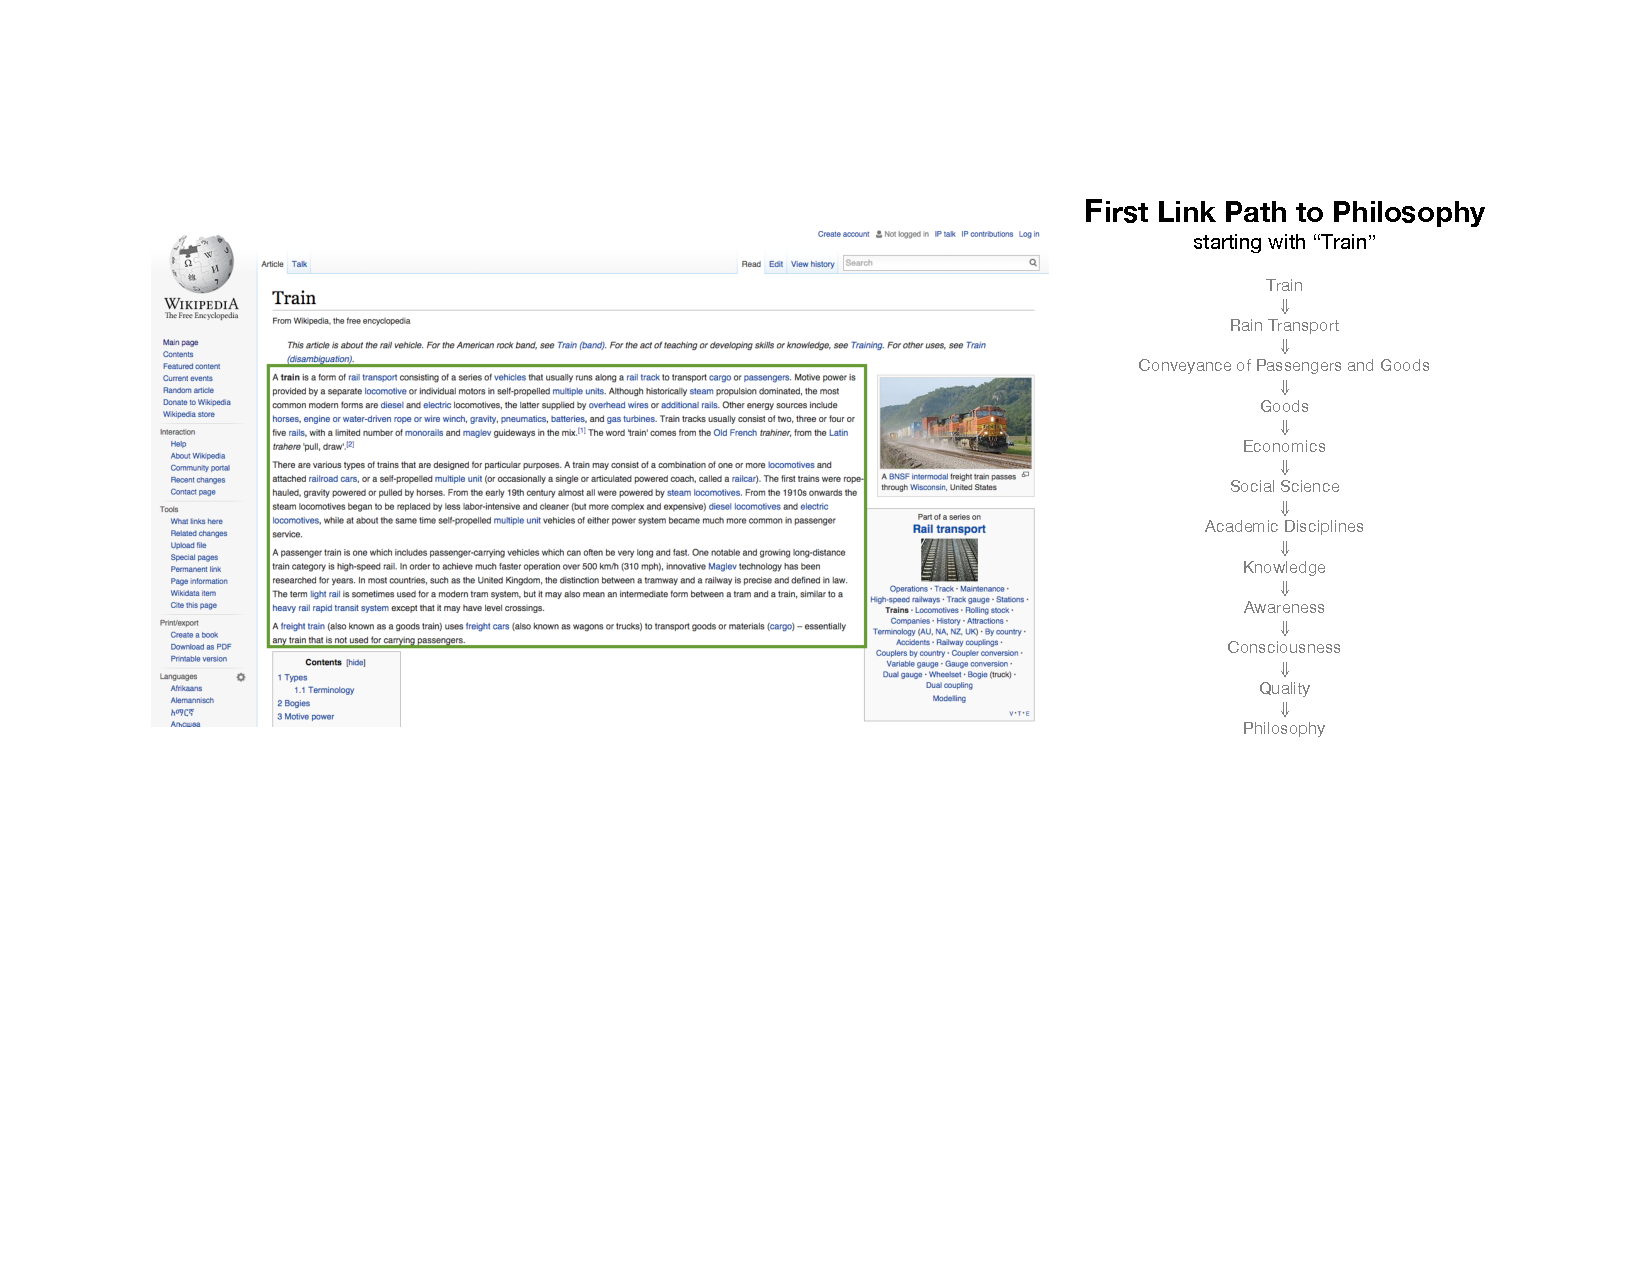
\includegraphics[width=\textwidth]{graphics/Train.pdf}  
  \caption{
    \textbf{First Link Path For "Train"}
    We follow the first link to another Wikipedia article
    in the main body of the article---the area
    inside the green rectangle, which excludes 
    side bar elements, the navigation bar and title. 
    In this example, the first link to another Wikipedia article is "Rail Transport." 
    We can again select the first link on the "Rail Transport"
    article, repeating the process to 
    form a path of First Links.
  }
  \label{fig:Train First Links}
\end{figure*}

What information could the first links possibly reveal?
Inspired by the claim that the majority of first links lead to the 
"Philosophy" article---popularized by an xkcd comic and subsequently
discussed in blog posts ---we holistically study 
Wikipedia's FLN as a map relating areas of human knowledge. 
The map is a hierarchical taxonomy where "Train" links to a parent node, 
"Rail Transport," while many child nodes, "Steel" and "Horsepower," link up to 
"Train." Unlike previous taxonomies
created by individuals
\cite{locke}
\cite{descartes}
\cite{aristotle} 
or a select group of individuals 
\cite{hist_thesaurus}, 
the organization of ideas in the FLN 
does not emerge from a concerted centralized effort, 
but rather from the independent choice of every article's authors.
The FLN is a wealth of relations among all the inventions, places,
figures, objects, and events described in Wikipedia, across space and time.


Our goal is to gain insight into how the information on Wikipedia is organized and related
by studying the structure of the FLN.
In a novel approach, we develop metrics to capture 
the dominant features of the FLN's structure.
We measure dynamics of the FLN as a flow, quantifying 
aspects of the FLN from the accumulation of first links around articles 
to the influence an article exerts in shaping the FLN.
Together with cycles, n-degree, depth, and the content of the articles, 
we build our analysis of the relations among the ideas in Wikipedia.


\section{Traversing the First Link Network}

To understand the structure of Wikipedia's First Link Network, we
aimed to characterize the dynamics of the flow from one article to another. 
Do links tend towards a particular article, group of articles, or groups of articles? 
What is the flow of links through a typical article?
What types of cycle (loop) structures exist in the network?
What are typical paths from one article to loop or an invalid link? 
Are there exceptionally long or short paths? 
Are there articles funneling the flow of links towards a particular path?
In answering these questions about the directed network, we aimed to characterize 
how so many independent articles relate to each other.


The n-degree, or number of links directly pointing to a particular article,
inadequately captures the dynamics needed to answer these questions.
The n-degree measures only the particular set of links to a particular article, 
rather than the richer dynamics of how the links flow through the network: 
where articles tend, what the typical and atypical 
paths through the network are, which articles funnel relatively more links and so on. 


Consequently, to capture the dynamics of how the First Links flow, we actually traverse every possible path through the FLN. 
The algorithm for traversing the network begins by selecting any article. 
We then proceed to the next article by following the First Link---recalling a First Link is a link in the main body of the article leading to another Wikipedia article. 
We repeat until the First Link is invalid or repeated to form a path. 
The collection of articles is path-connected conveying a flow of concepts from one article to another. 
The method is order agnostic with respect to which articles are selected first.
As long as each article is selected eventually, the resulting metrics are equivalent.

We developed three metrics to uncover structure: 
traversal visits, traversal funnels, and path length. 
Each metric captures one essence of how the links flow. 
Traversal visits gauge the accumulation of links; 
traversal funnels gauge the influence on link path; 
path length measures the number of First Links to a repeated or invalid link. 


\begin{figure*}[tp!]
  \centering	
  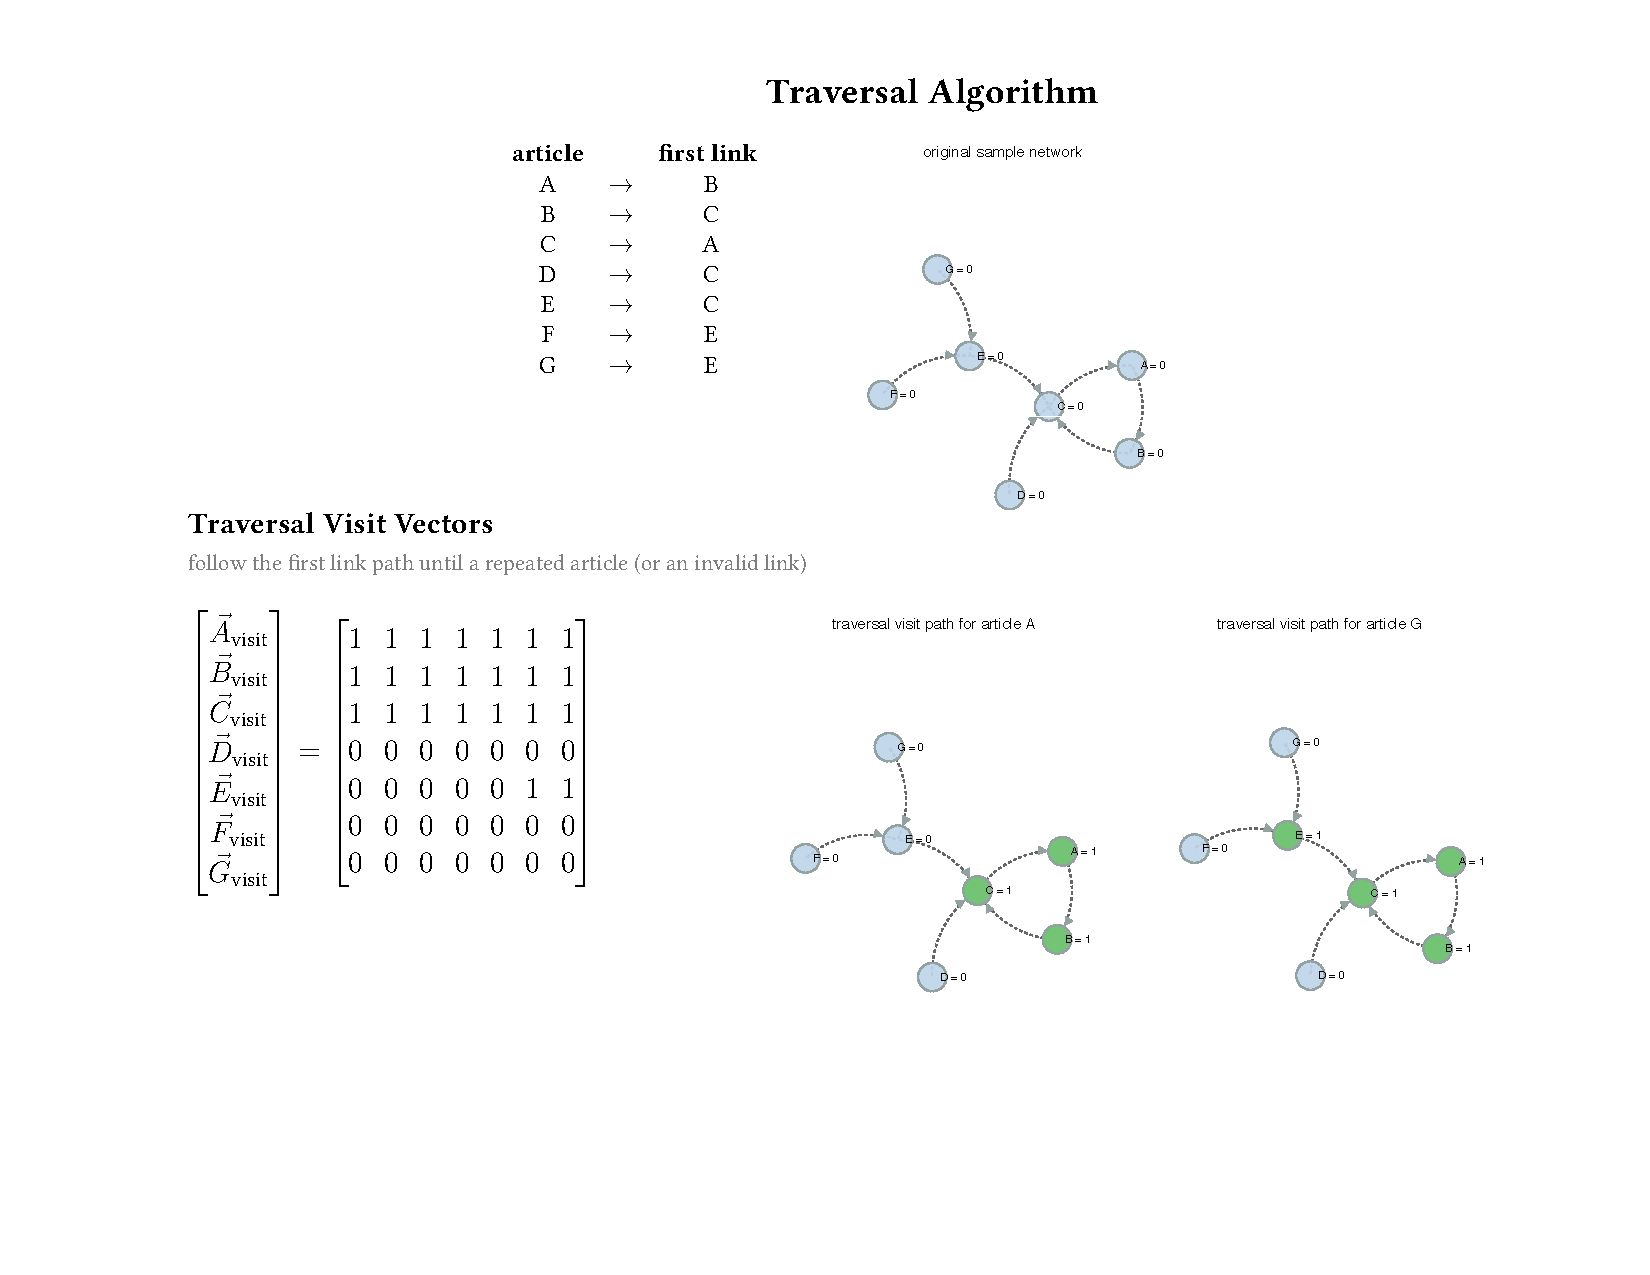
\includegraphics[width=\textwidth]{graphics/traversal_visit_algo_figure.pdf}  
  \caption{
    \textbf{Traversal Visit Algorithm on a sample network}
     The traversal visit vectors are an adjacency matrix for the paths through the network: the first column is indicates the path formed starting with article A. The number of traversal visits for article A is then the number of paths containing A or the sum of the first row in our matrix:
     $\sum_{i=1}^7 A_{\text{visit, i}} = 7$.
  }
  \label{fig:Traversal Visits}
\end{figure*}

The first metric, {\it traversal} visits, gauges where the flow of first accumulates by associating a count to each article. 
Every path through the article increments the associated count by one. We can construct a vector to represent the articles incremented on a particular path, combining these vectors to form a matrix. 
The total accumulated counts for a given article is then simply the sum of the row in our matrix corresponding to the article of interest. 
Node A in our example (see figure ~\ref{fig:Traversal Visits}) has 7 traversal visits, since every path includes article A. 
Whereas, node E only has two traversal visits since only two paths contain article E for example.
What we have then is a metric signaling which article contains a larger accumulation of first links.


While traversal visits measure accumulation, we cannot gauge whether a particular article exerts a greater influence on flow of the first link paths. 
To distinguish between an article that simply happened to fall within a cycle from an article actually funneling the flow of first links, we developed a second metric called traversal funnels. 
We traverse the network in the same manner, but end our paths once we enter a cycle. 
We again increment the associated count of each article by one if the path up to a cycle contains the article. 
We call the accumulated count the number of {\it traversal funnels}. By measuring traversal funnels, we quantify
which articles funnel more link paths in a particular direction or cycle 
(see figure ~\ref{fig:Traversal Funnels})
.

\begin{figure*}[tp!]
  \centering	
  \includegraphics[width=\columnwidth]{graphics/traversal_funnel_algo_figure.pdf}
  \caption{
    \textbf{Traversal Funnel Algorithm on a sample network}
  The algorithm for traversal funnels is identical to the previous algorithm for traversal visits with one alteration: the path ends at the start of a cycle to distinguish articles directing a path into a cycle from articles that simply happen to be in a highly traversed path. We can construct similar vectors by considering each path through the network, measuring traversal funnels for a particular article as the sum of the entries in its corresponding row. For example
  the number of traversal funnels for article $E$ is 
  $\sum_{i=1}^7 E_{\text{funnel, i}} = 2$.}
  \label{fig:Traversal Funnels}

\end{figure*}

Finally, we track the number of links until a repeated article or invalid link, to find the typical path length within the network.
By recording the history of articles we traversed, we are also able to uncover several other network characteristics including basins, defined as a collection of path-connected articles ranked by traversal visits, and cycles of various lengths.
The three metrics: traversal visits, traversals funnels, and path length, along with our path history
yield a powerful arsenal of information with which to study the network. 


\section{Discoveries}

We followed every possible path through the network, taking 232 million steps along the way to measure the accumulated number of traversal visits.

\subsection{Traversal Visits}

As a distribution, the number traversal visits per article appears scale-free. The majority of articles have fewer than 30 traversal visits, while few 
have 5 order of magnitude more traversal visits. 
Specifically, $99.76\%$ of articles have fewer than $100$ traversal visits; nearly $80\%$ have none. 
Meanwhile, the highest ranking 30 articles have an extremely disproportionate number of traversal visits.

\begin{figure*}[tp!]
  \centering	
  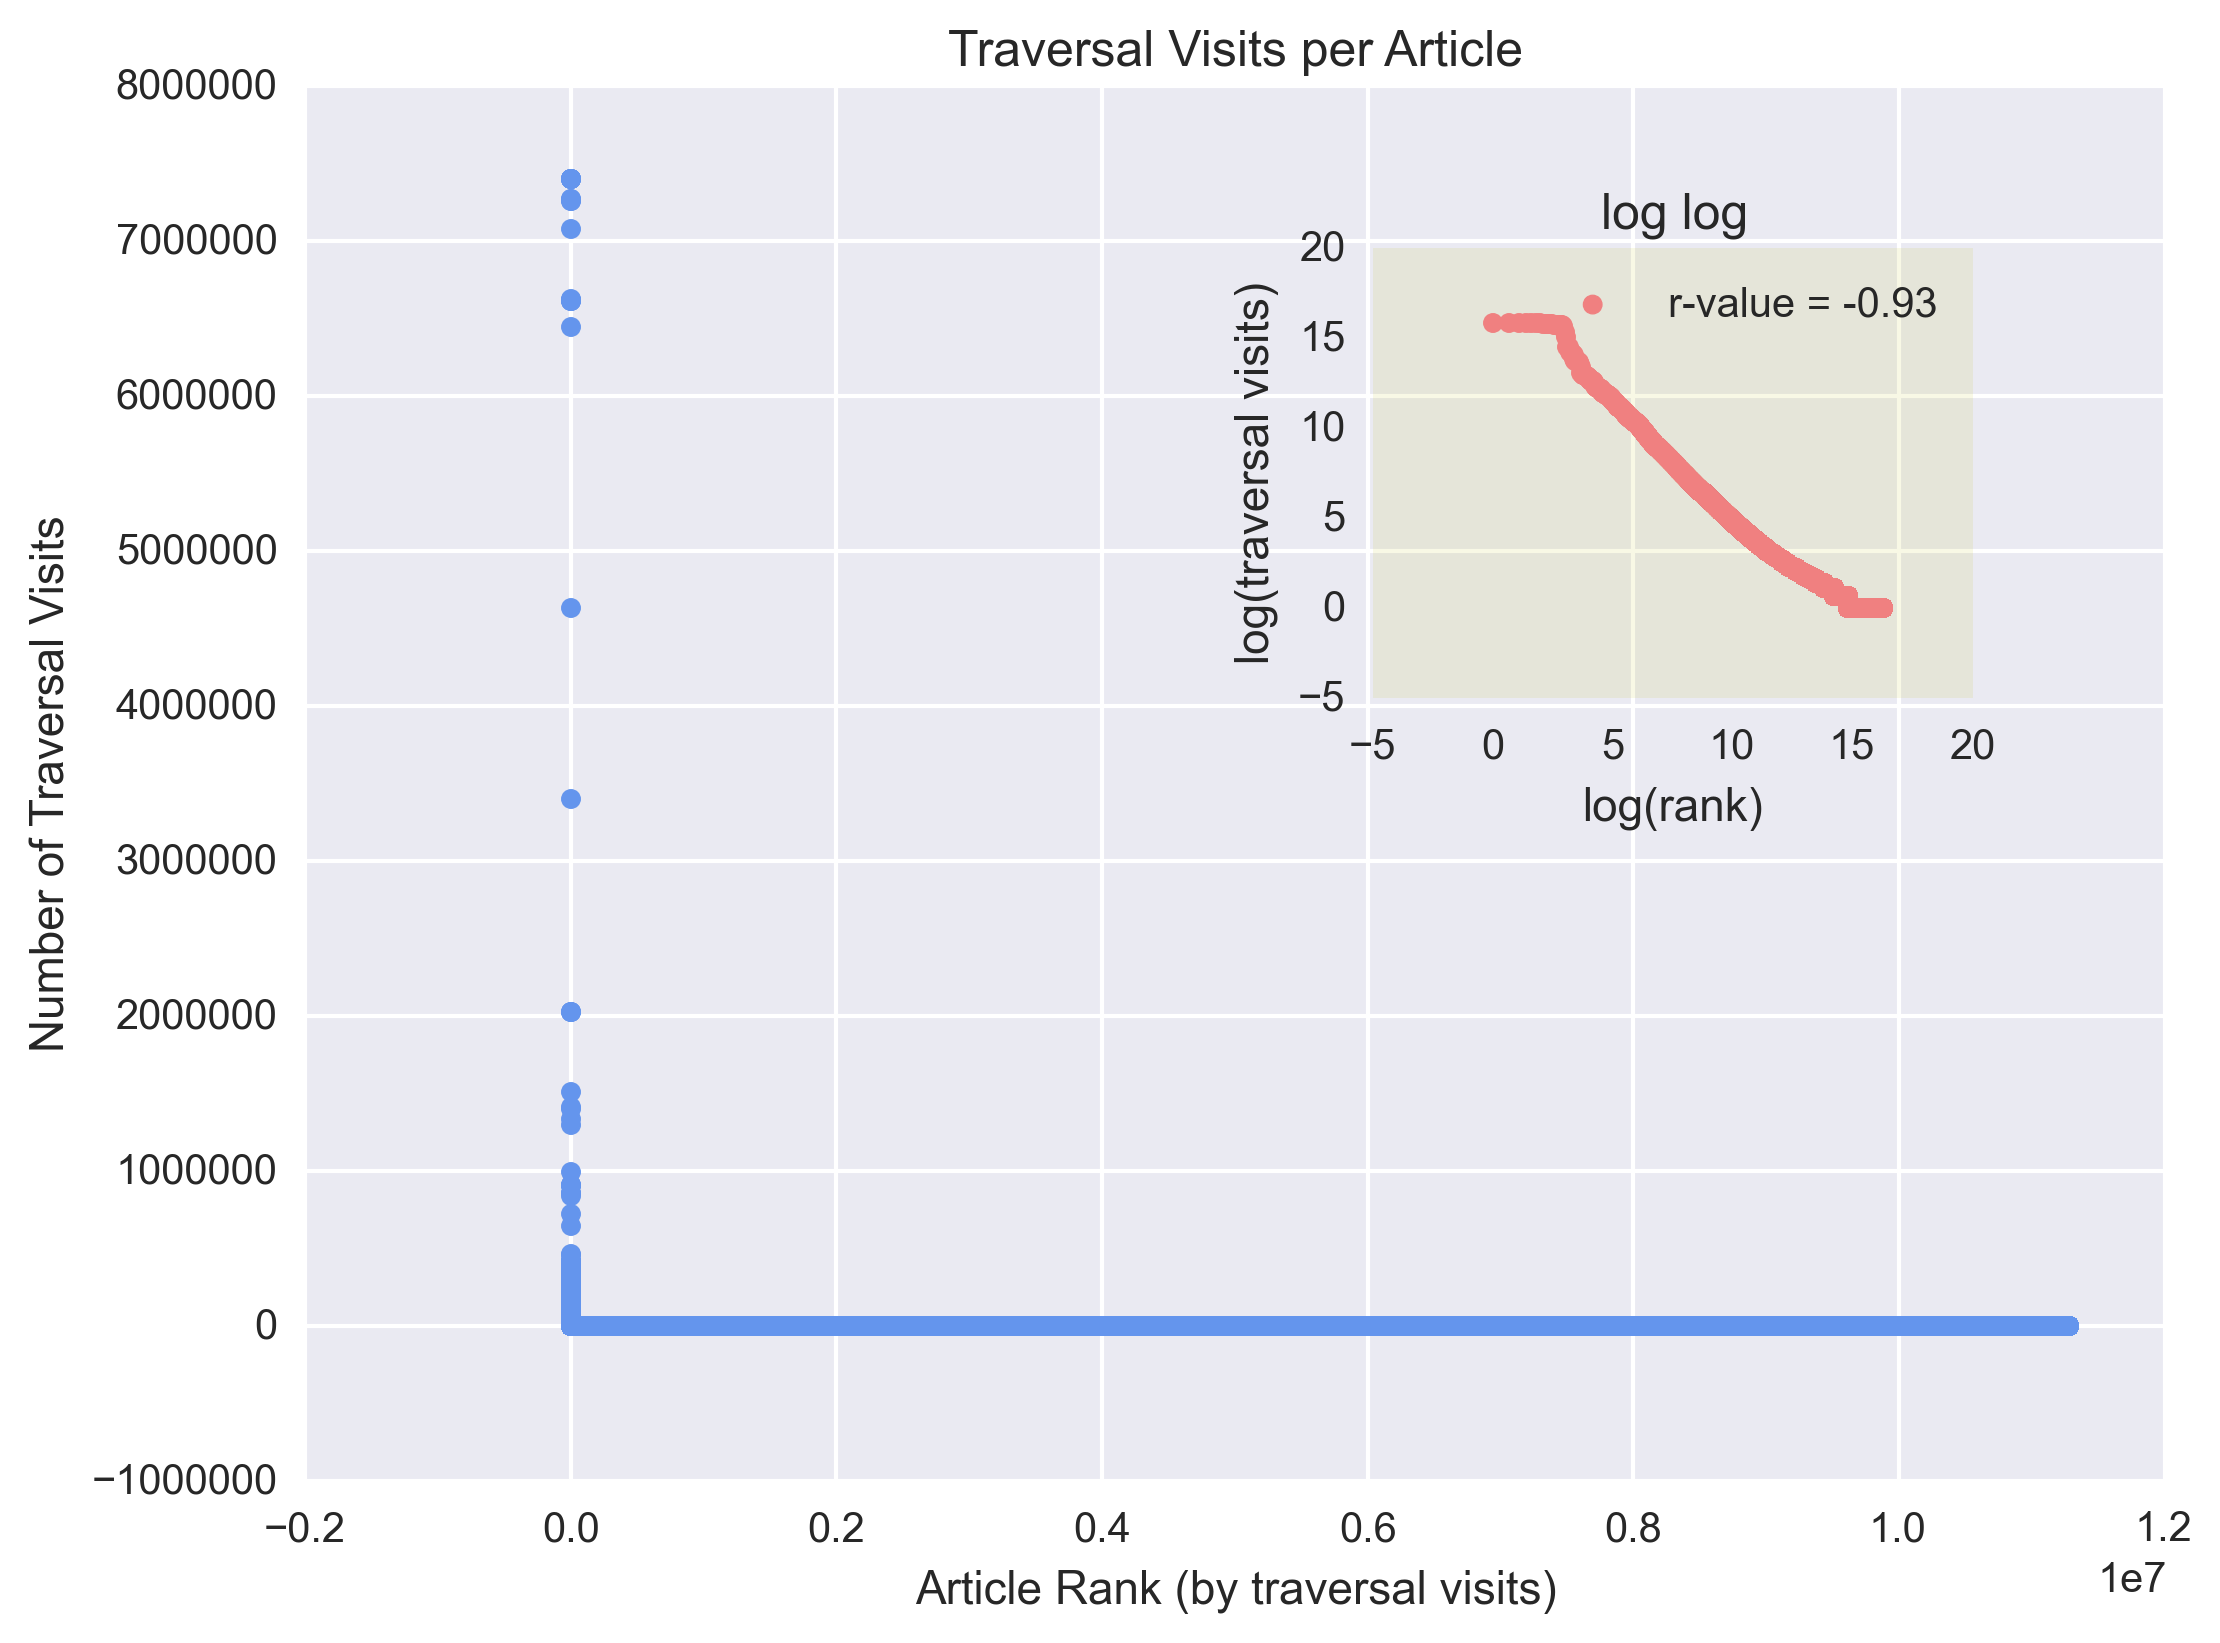
\includegraphics[width=\columnwidth]{graphics/traversals_per_article.png} 
  \caption{
    \textbf{Distribution of Traversal Visits}
  }
  We fit the distribution to a linear log-log model by considering the log (base 10) transformed rank of each article against log (base 10) transformed the number of traversal visits. 
  The model explains $86\%$ of the variation in the data, yielding an r-value of $-0.93$ 
  and a power law exponent of $-0.636$. The horizontal flattening around the highest
  ranking articles is a result of the cyclic structure (see discussion on cycles).
  \label{fig:Distribution of Visits}

\end{figure*}

To more accurately gauge the distribution, we construct a log-log plot of the entire dataset: log(traversal visits) against log(rank). We observe a fairly linear fit, as is characteristic of scale-free networks, with an r-value of -.93 and 
a power-law exponent of $-0.636$. A handful of the highest ranking articles contain a disproportionate number of traversal visits, while most have none. The skew in the distribution is not terribly surprising when considering the heuristic of how the links flow: from specific to general. 

The highest ranking articles include Philosophy alongside related articles such as "Existence", "Quality", and "Reality".

\begin{figure*}[tp!]
  \centering	
  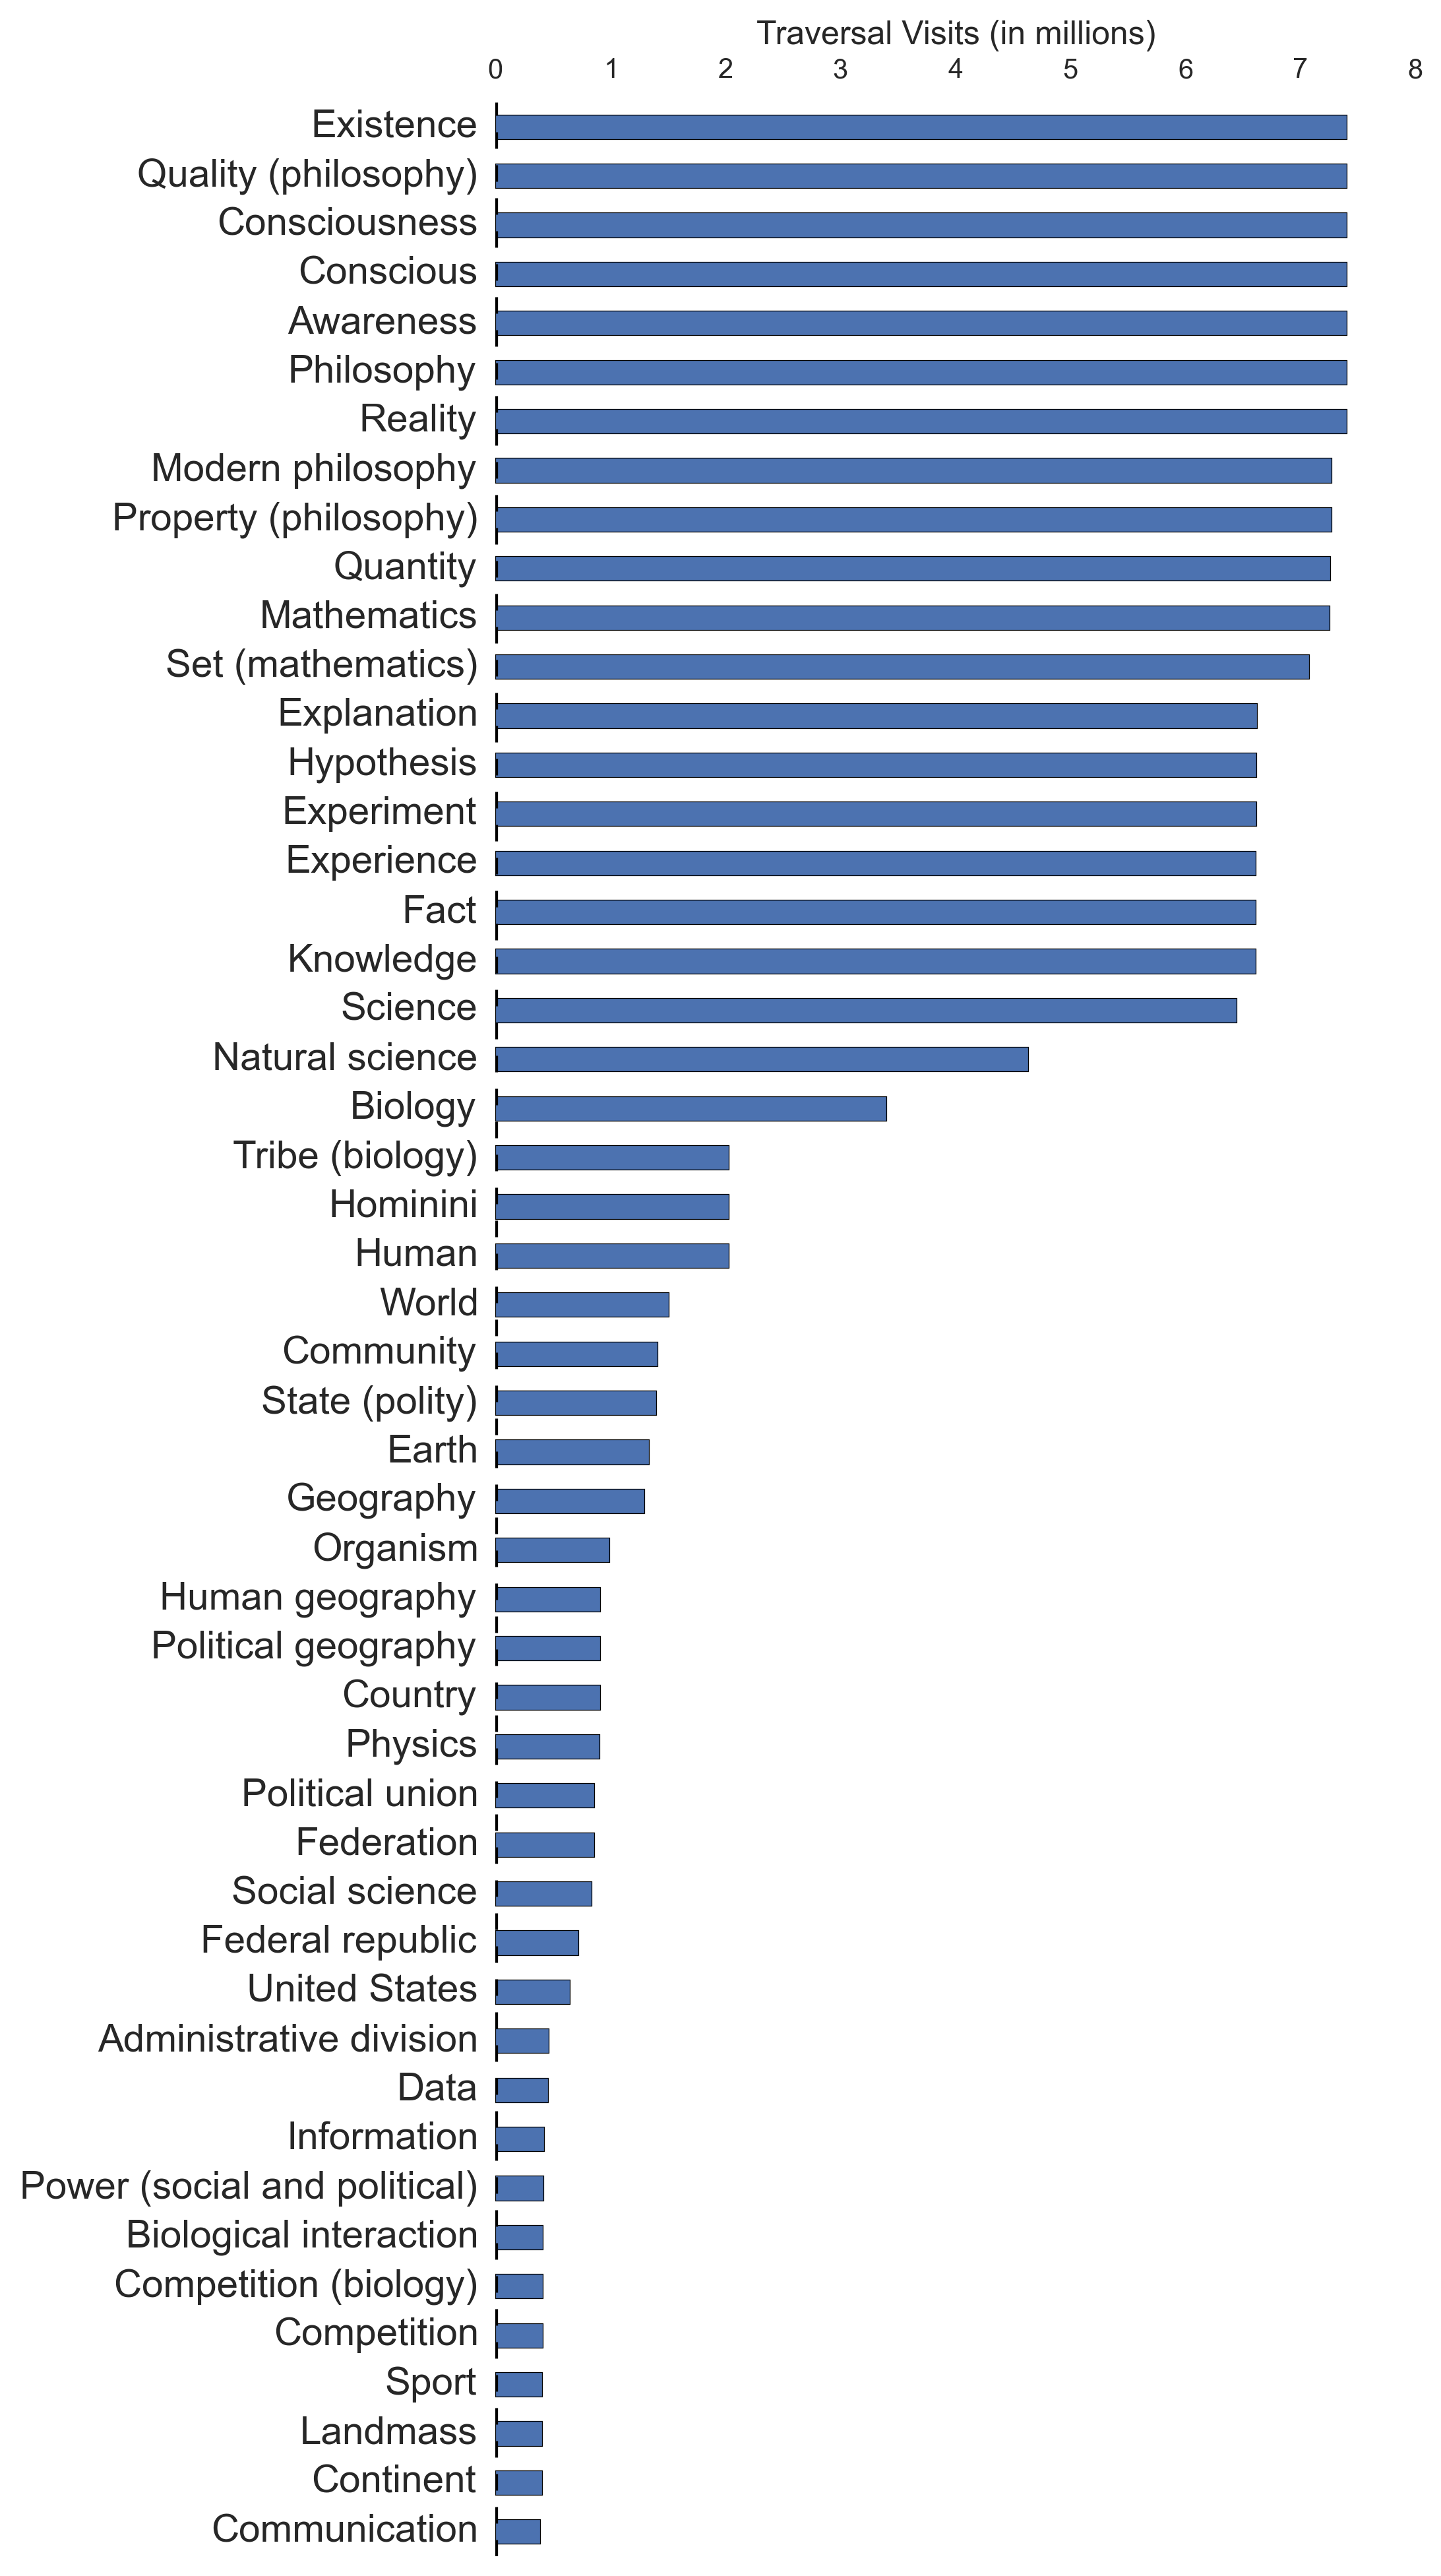
\includegraphics[width=\columnwidth]{graphics/articles_ranked.png}
  \caption{
    \textbf{highest ranking articles by number of traversal visits}
  }
  We compute the number of traversal visits for each article in the FLN (see 
  Traversal Algorithm section for details). In doing so, we can rank each article
  by the accumulation of first links. Articles with a greater number of traversal visits
  mark greater points of first link accumulation. The highest ranking articles by traversal visits reveals where the greatest accumulation occurs.
  \label{fig:highest visits}
\end{figure*}


\subsubsection{A flow from general to specific}

The highest ranking articles by traversal visits are 
broad, global topics: 
many are academic disciplines such as "Science," "Math," 
"Geography," "Biology," and "Physics"; others are abstract fundamental concepts such as 
"Community", "State", "Earth", "Information", "Communication", and "Power."
Since traversal visits measure the accumulation of First Link visits in Wikipedia, 
the highest ranking articles suggest a flow from specific to general. 
For example the flow of First Links for the "Banana" article begins at a very concrete
and specific topic then flows into progressively broader and broader disciplines, eventually 
culminating at "Philosophy: "Banana" links to the broader category of "Fruit," which then links to 
"Botany," eventually "Biology," then "Science" and ultimately "Philosophy." 

One means to measure the specificity of an article is to identify the number of synonyms available for a word or topic. The reasoning here is that a  broader topic likely has many more synonyms relative to a specific, concrete topic. Banana has fewer synonyms than botanical for example. To quantify the observed flow, we measured the number of synonyms the article title contained in WordNet---the largest lexical database of the English language. We find the highest ranking 100 articles have on average 5 more synonyms than the typical article; a difference of 2.5 synonyms if we compare the median number of synonyms in each group. As suggested by the median, many articles have no synonyms as we might expect, because titles with more than one word are not likely to appear in a thesaurus. Since many articles have no synonyms, we also compared the number of synonyms in the highest-ranking versus typical article, this time excluding all articles without at least 1 synonym. We still find the highest ranking 100 articles with an average of 9.0 (median of 7.0) synonyms whereas the remaining articles on average 5.8 synonyms (median of 7.0), even with the exclusion of all articles without any synonyms.
The quantifiable difference in synonyms corroborates the flow of links from concrete, specific articles to broader disciplines or fundamental notions.




\subsection{Network Cycles}

The recurrence of an exact number of traversal visits suggests some articles are part of a cycle. 
The "Philosophy" article for example sits in what seems like a cycle of seven other articles; "Hypothesis" appears to sit in a 
cycle of 6 other articles including "Experiment", "Fact", and "Knowledge".
To confirm the suggested cycle structure, we recorded the history of articles traversed along a path. 

We first identified 2-cycles, meaning a pair of articles with First Link pointing to one another.
Of the 11 million articles, 84,000 are 2-cycles. 
The highest ranking 2-cycles by traversal visits tend to be synonyms (or nearly so) rather than different, yet connected ideas:
"Health Care" and "Medical Case Management", "Broadcasting House" and "BBC", "Secondary Education" and "Secondary School".

\begin{figure*}[tp!]
  \centering	
  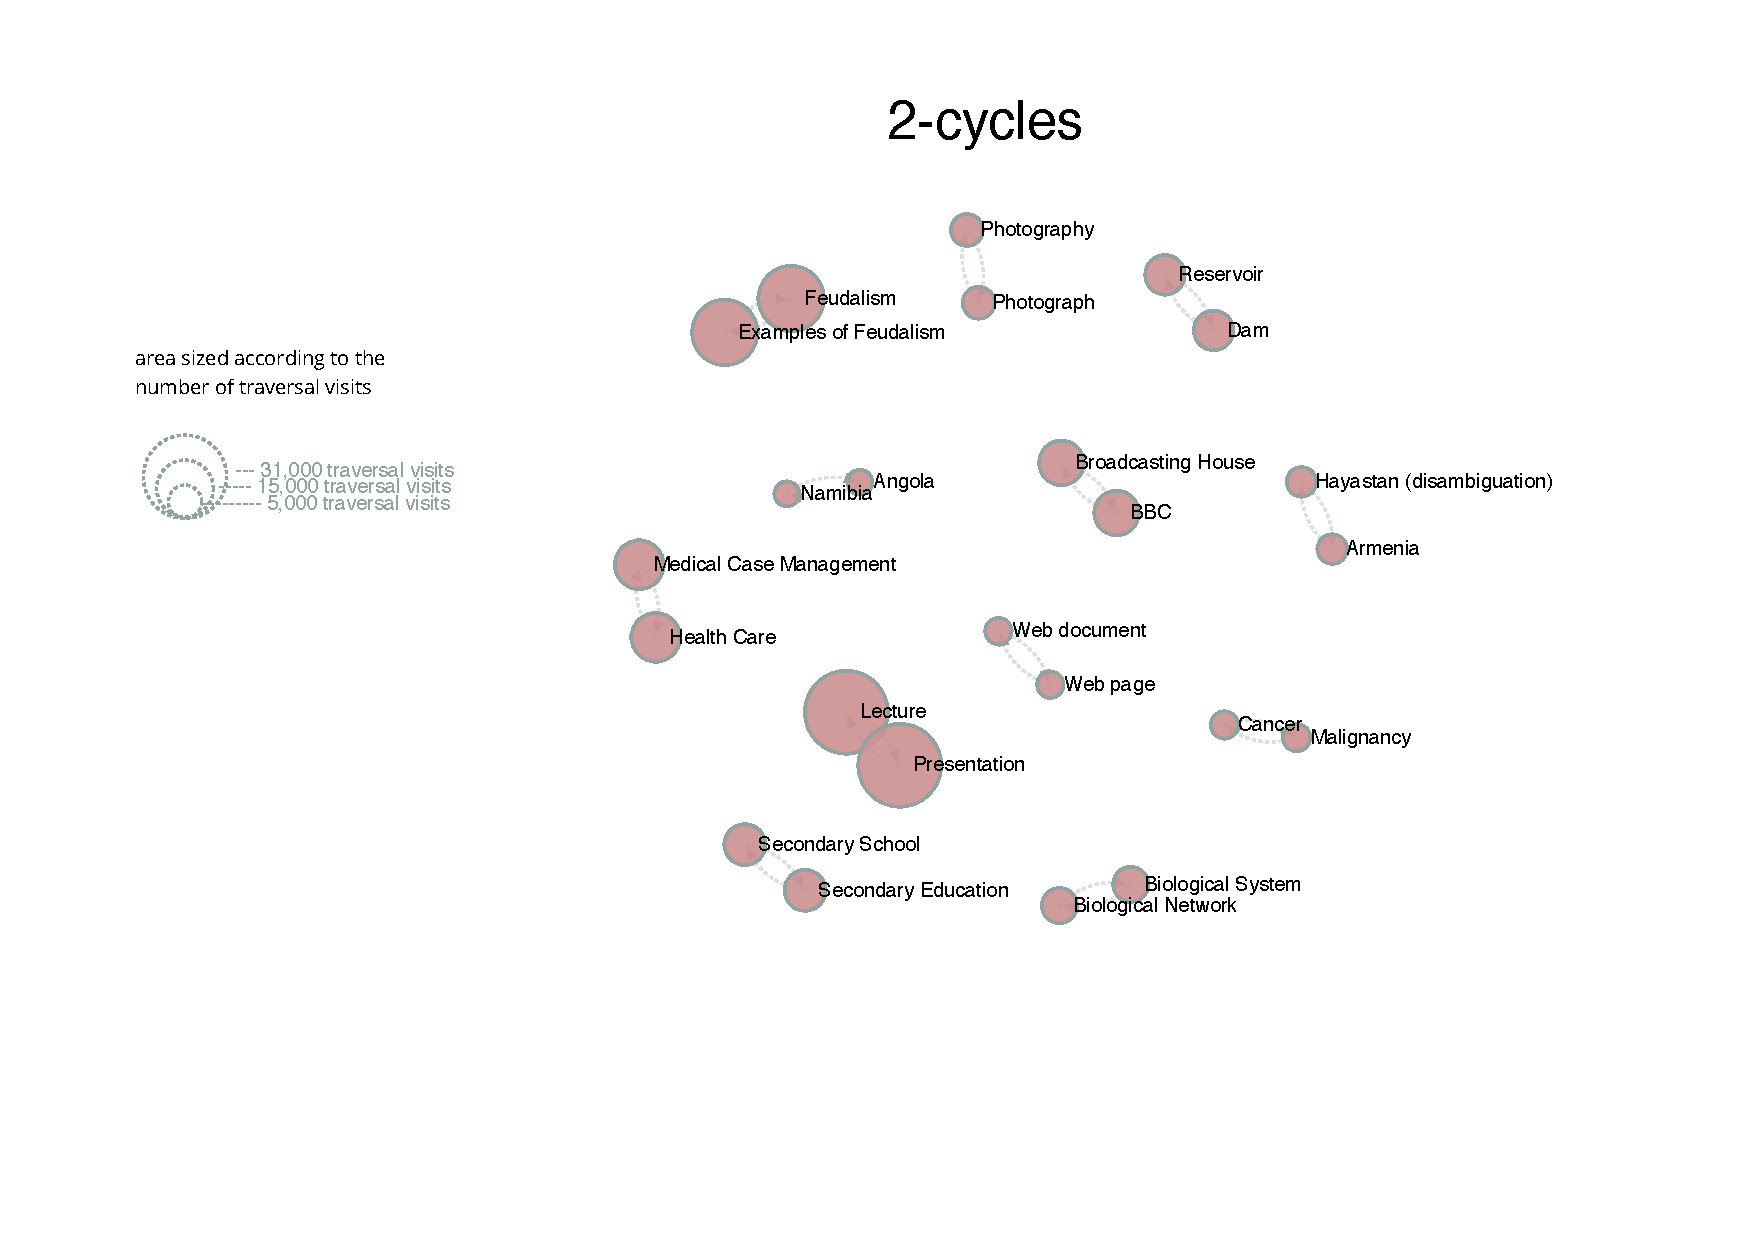
\includegraphics[width=\textwidth]{graphics/2_cycles.pdf}
  \caption{
    \textbf{highest ranking 2-cycles}
  }
  \label{fig:2-cycles}

\end{figure*}

Outside of the highest ranking 2-cycles, the typical 2-cycle signals a connection between different, yet very closely related ideas. 
Link patterns such as inventor to product ("Voere" to "VEC-91"), event to organizer ("Poetry Bus Tour" to "Weave Books"), and book to author ("Anatomy of Britain" to "Anthony Sampson").

Similarly, 3-cycles captured a synonymous or close relation among 3 articles: "Tree of life (Biology)", "Tree of life (disambiguation)", 
and "Tree of life"; "Cinema of India", "Indian Cinema", and "Telugu Cinema". Once we extend our cycle size beyond a length of 6 however, 
"Philosophy" along with the remaining list of high ranking articles by traversal visits dominate.

\begin{figure*}[tp!]
  \centering	
  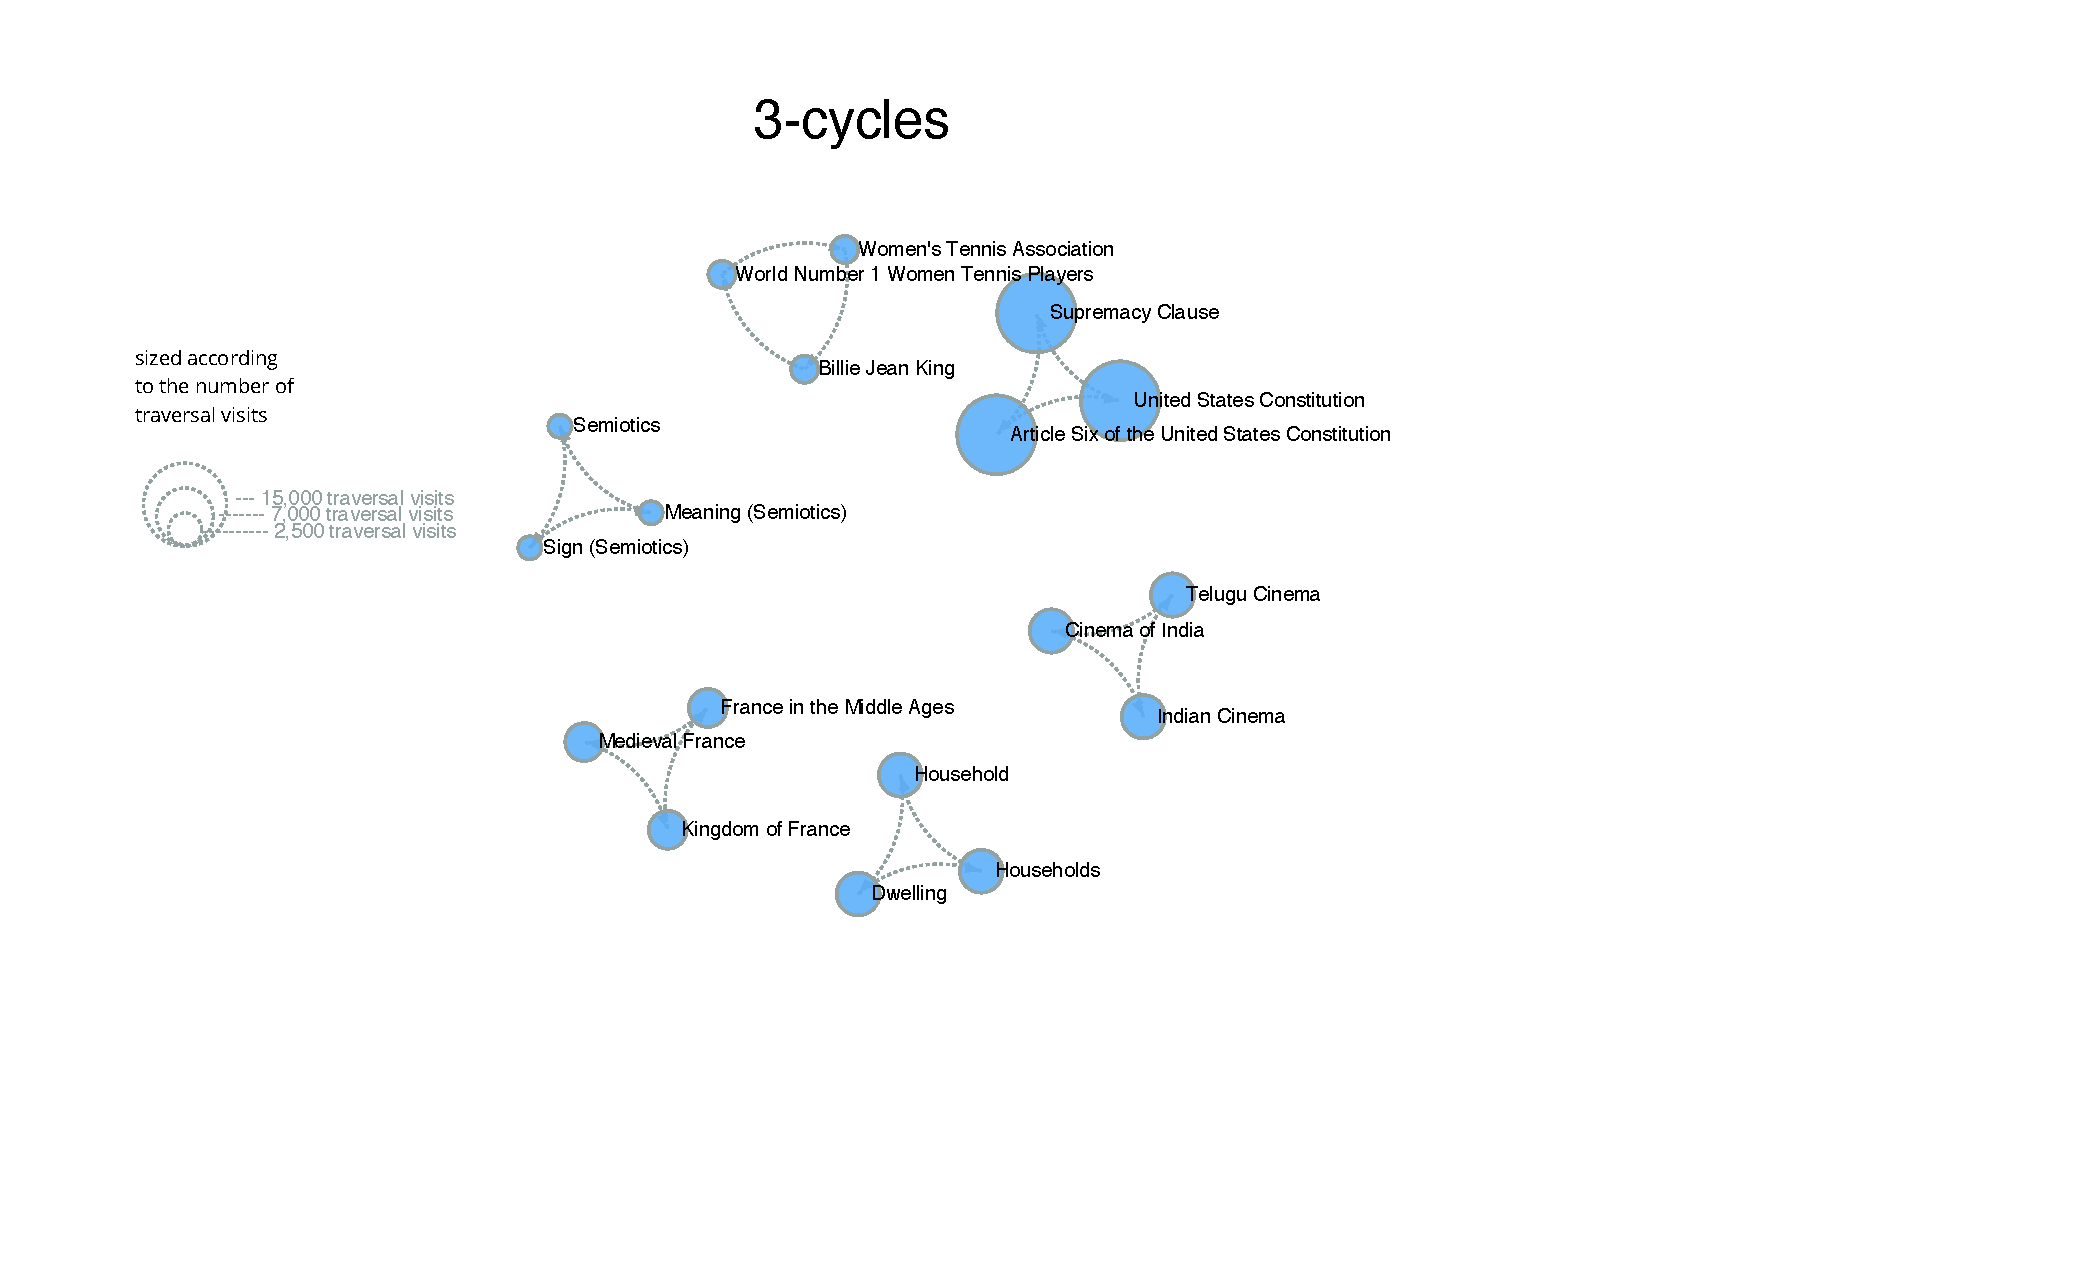
\includegraphics[width=\textwidth]{graphics/3_cycles.pdf}
  \caption{
    \textbf{highest ranking 3-cycles}
  }
  \label{fig:3-cycles}
\end{figure*}

The longest cycle in the network spans 365 articles of Eastern Orthodox Liturgics for each calendar day. 
Curiously, on the last calendar day, the last article simply links back to January 1, forming a 365-cycle.
Other lengthy cycles span 60-75 articles including collections of articles on national histories such as "Japanese Eras" 
or judicial bodies such as the "Legislative Assembly of Ontario".





\subsection{Basins}

We can group articles lying on the same path to identify {\it basins}: 
a group of path-connected articles.
Since cycles identify only groups of articles with a closed set of links, 
we additionally measure and rank basins to capture groups of closely related
articles branching outside of a cycle into the rest of the FLN.
Akin to river networks, these basins are areas of FLN accumulation with a path 
flowing outwards to the rest of the FLN.
The highest ranking basins by the number of traversal visits are groups of articles
around "Philosophy" given the high number of traversal visits "Philosophy" has. 
However, restricting our attention to the 
 single articles around which basins formed,
 we find high ranking basins around similarly foundational ideas:
"Community", "Landmass", "Federal Government", "Presentation", and "Belief System". 
Around each article is a sets of related ideas. Around "community" are groups of articles expressing similar ideas: "Political Union," "State," and "Federation." 
These concepts naturally emerge from the First Link Network potentially indicating pillars, which 
anchor specific knowledge in a broader, simpler concept.

\begin{figure*}[tp!]
  \centering	
  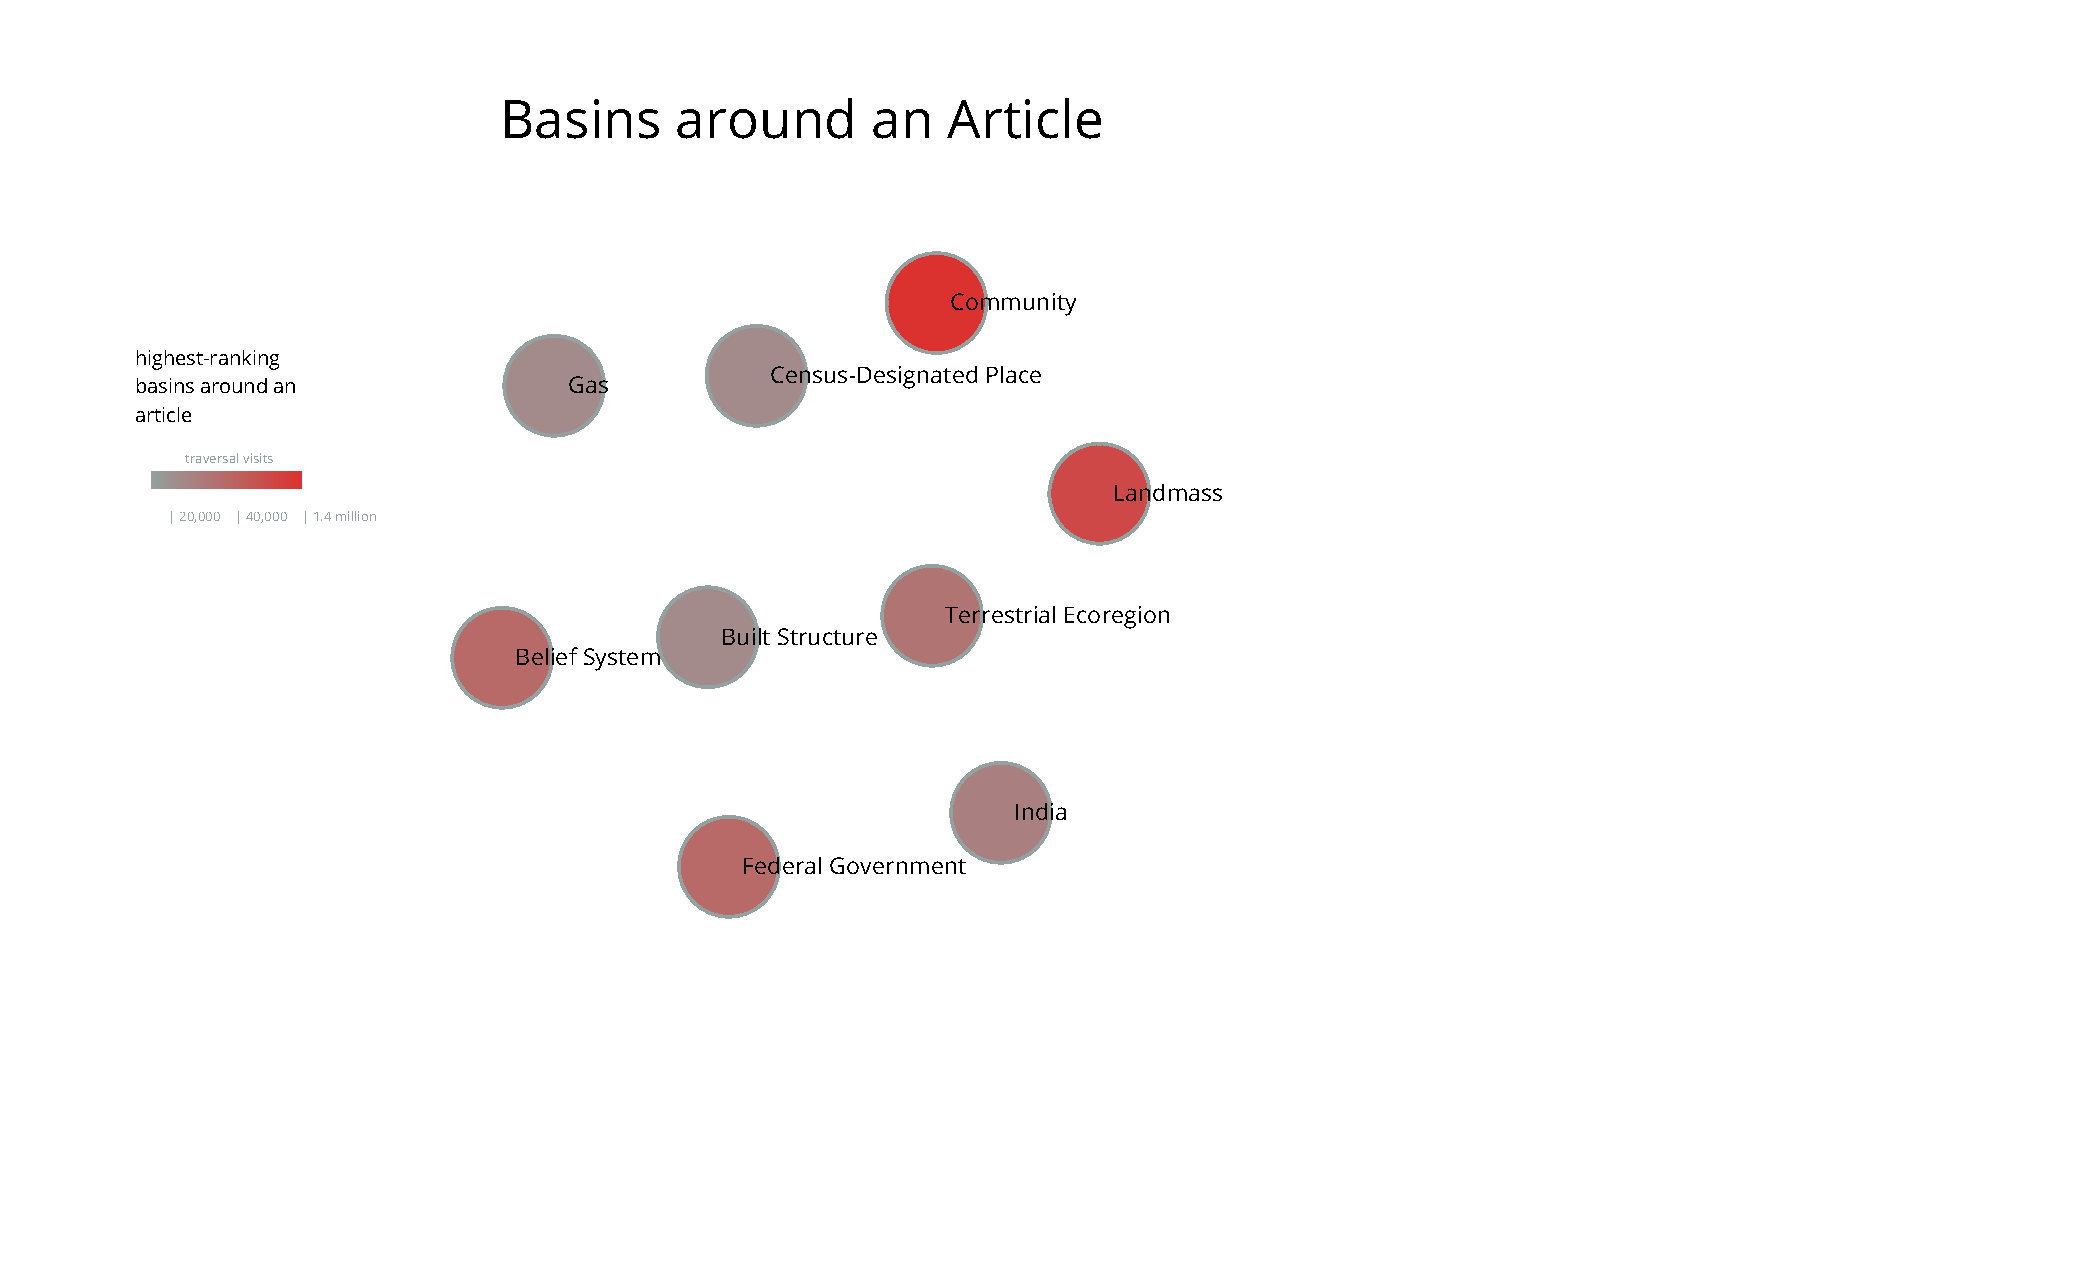
\includegraphics[width=\columnwidth]{graphics/basins.pdf}
  \caption{
    \textbf{basins around a single article}
  }
  \label{fig:basins}

\end{figure*}

\subsection{Path Length}

In addition to identifying cycles and cycle lengths, we also measure the traversal path length, which includes articles outside
of cycles. 
Path length measures the number of links traversed until a repeated or invalid link. 
We discovered the longest path length is also 365, matching the longest cycle of Orthodox Liturgics. 
We also found similarly lengthy paths following the evolution of a place or topic through time: 
"1953 in Scotland" or "1560s Architecture", with articles sequentially proceeding by year, decade or era.

Of the 11 million articles, 5.5 million had an invalid link or linked back to the same article, yielding a path length of zero. 
The most common path length is 29, with an interquartile range (26, 30).
The distribution of path lengths is similarly scale-free with few articles at the extreme of 365 path lengths, while the majority 
is between 26-30: 

\begin{figure}[tp!]
  \centering	
  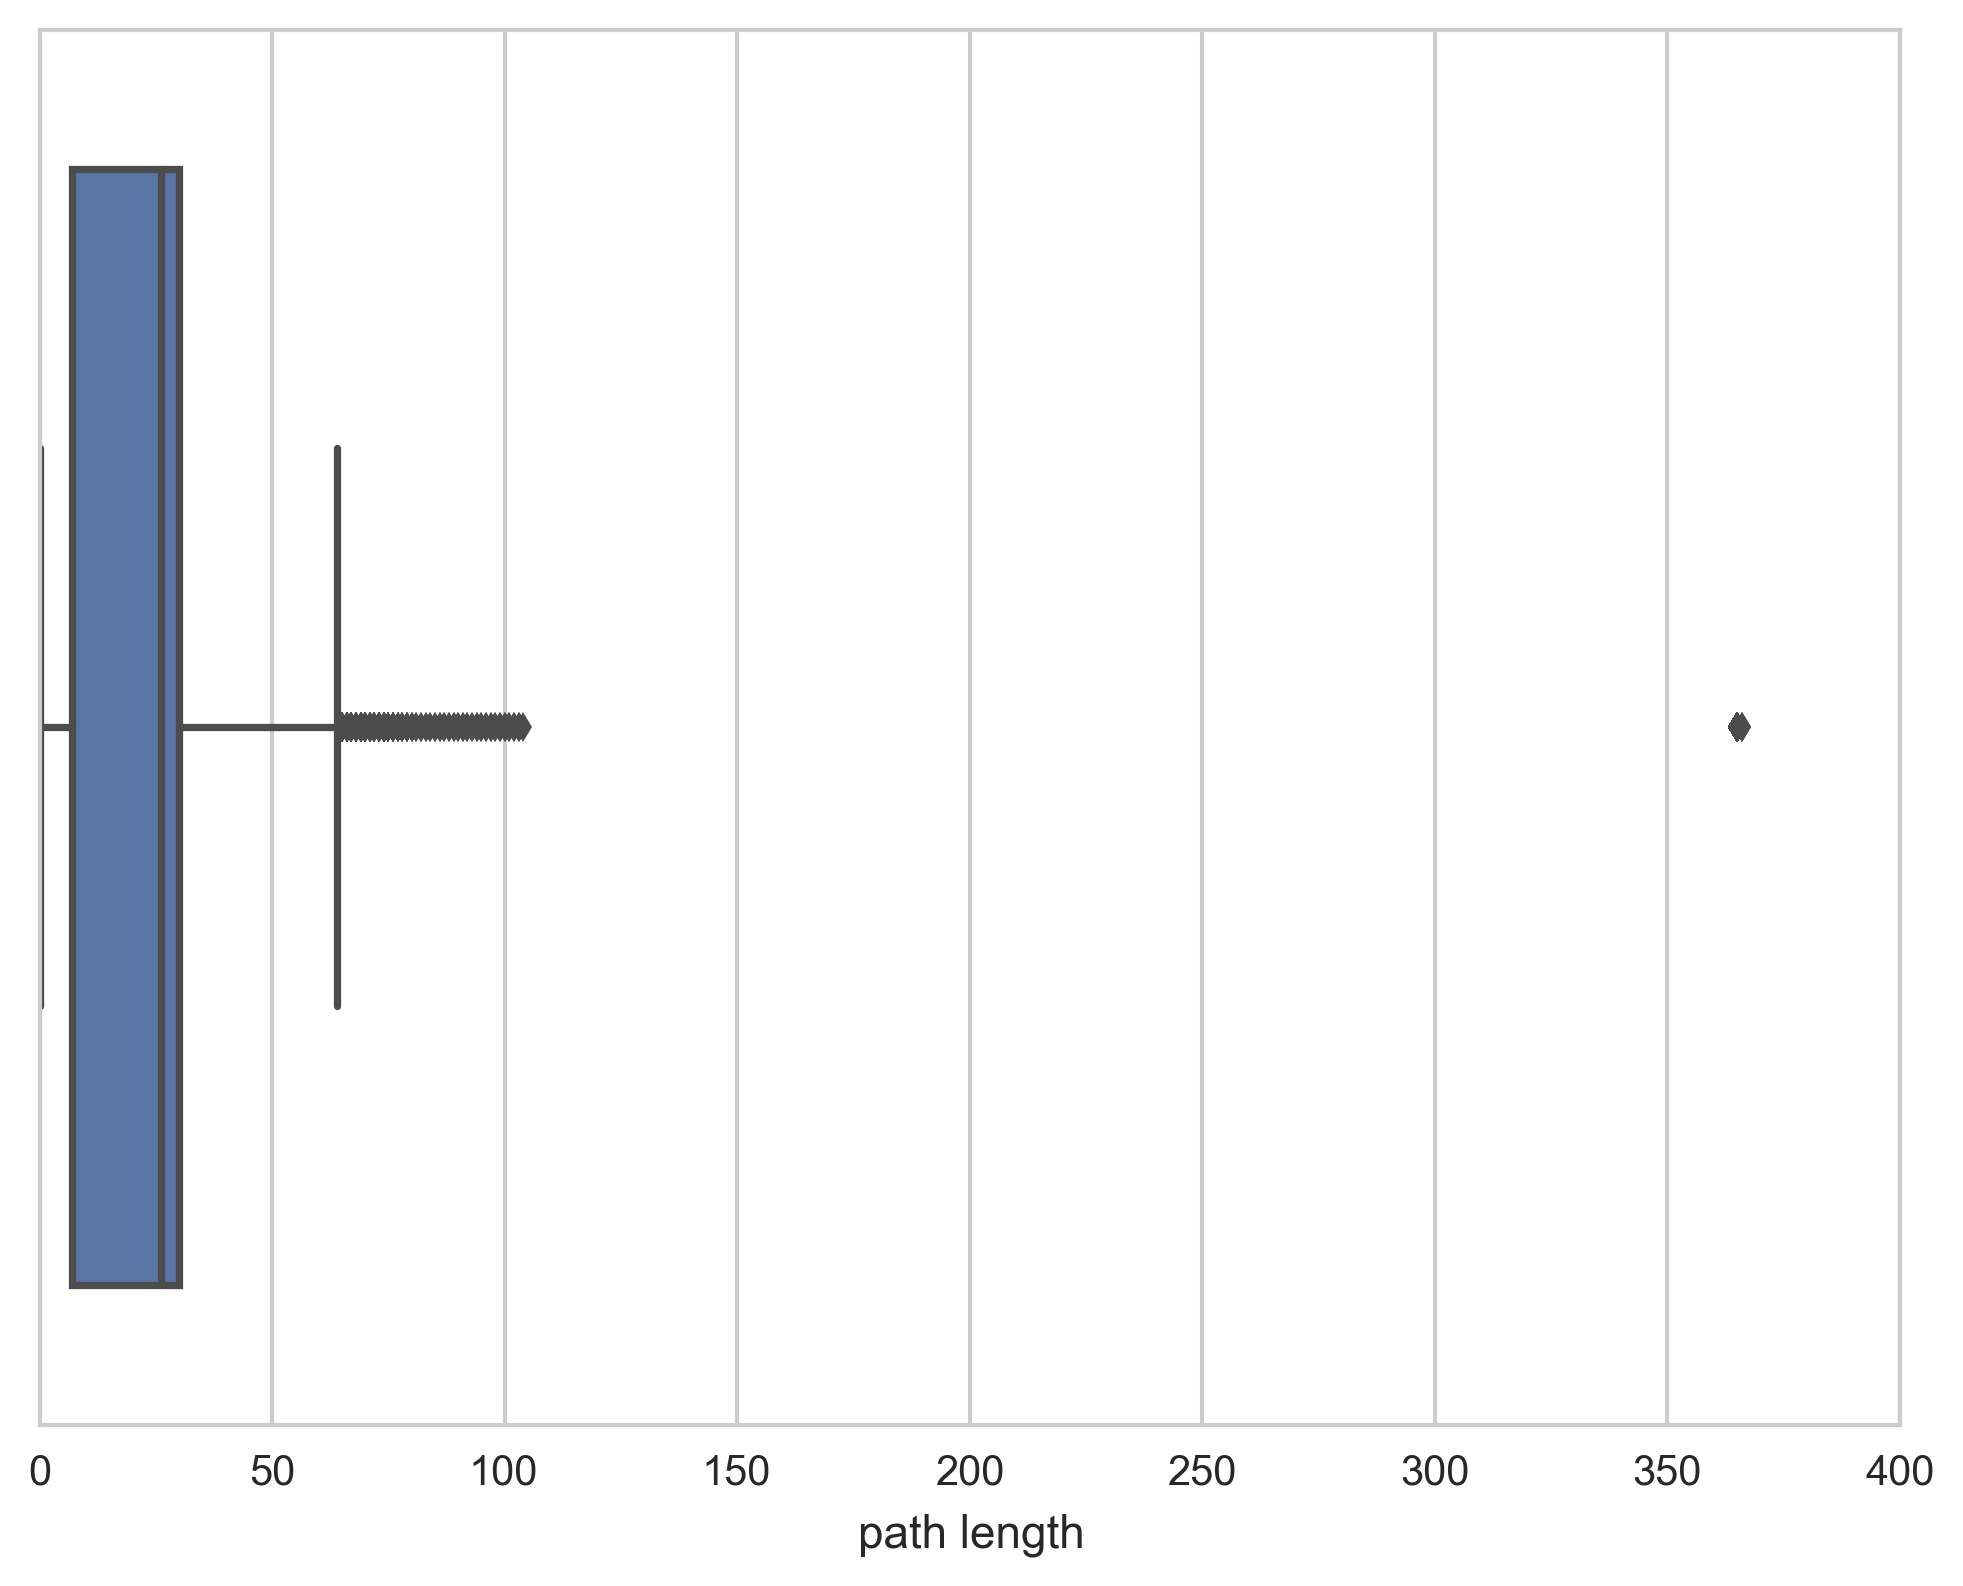
\includegraphics[width=\columnwidth]{graphics/path_lengths_boxplot.png}
  \caption{
    \textbf{Path Length Distribution}
  }
  \label{fig:Path Length Distribution}
\end{figure}

\begin{figure*}[tp!]
  \centering	
  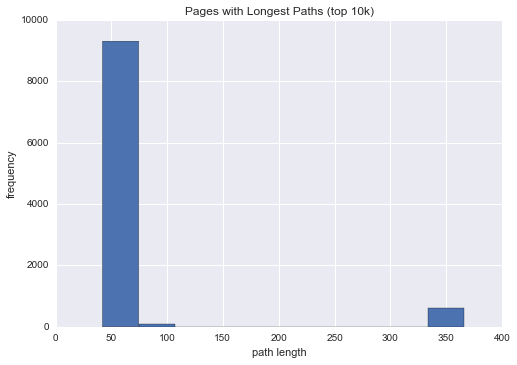
\includegraphics[width=\columnwidth]{graphics/top_1k_path_length.png}  
  \caption{
    \textbf{Path Length Distribution for Top 1k articles}
  }
  \label{fig:Top 1k Path Length Distribution}
\end{figure*}


\subsection{Degree Distribution}

We identified the set of first links directly referencing each article. 
Similar to the number of visits, we can examine the overall distribution and 
first links to understand the direct structure of taking one step through the 
FLN. 


\begin{figure*}[tp!]
  \centering	
  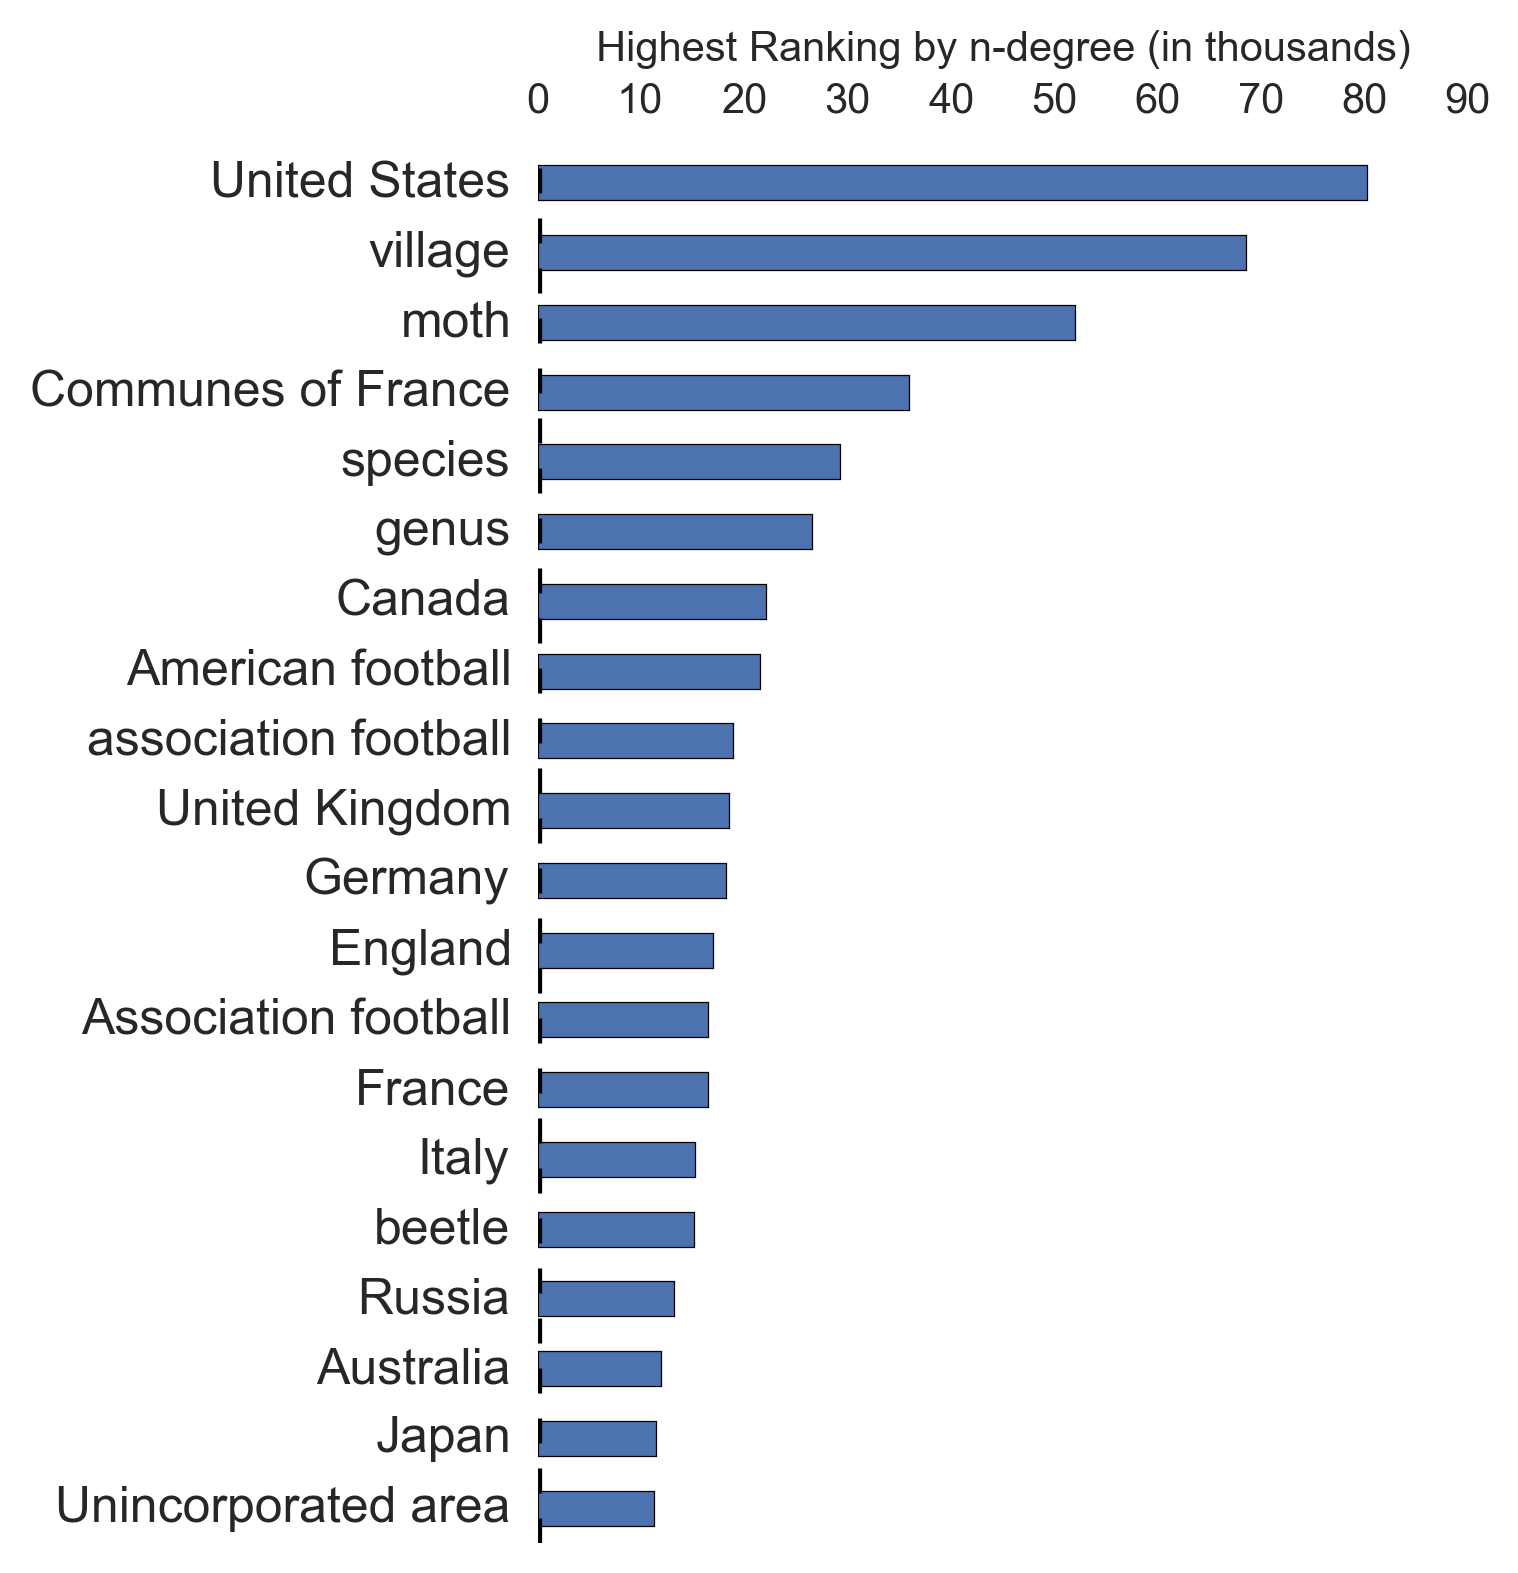
\includegraphics[width=\columnwidth]{graphics/articles_ndegree.png}
  \caption{
    \textbf{Highest Ranking Articles by n-degree}
  }
  We rank each article by the number of direct first links to the article (n-degree). 
  \label{fig:ndegree list}

\end{figure*}
The highest ranking article by n-degree, or the number of direct first links, is 
"United States" with 80,249 direct first links. Other high-ranking articles
include foundational abstract concepts such as "village," "species,"; 
sports associations such as "American Football," "Association Football"; 
and developed nations such as "France," "Japan," "Russia," "Australia," and 
the "Netherlands." 

"Philosophy" and other Philosophical concepts which hold many traversal visits,
do not appear near the top when ranked by n-degree. 
"Philosophy" has an n-degree of 581, with direct first links from articles about Philosophers and areas of Philosophy: "Existentialism and Humanism," "Predeterminism," "Synoptic Philosophy,"Qualia," "Dorothy Emmet," and "Christopher W. Morris."
While many articles accumulate at "Philosophy," the accumulation is not the 
result of many articles directly referencing "Philosophy." 
Instead, the accumulation of first links, as we argued in our 
discussion of traversal visits, flows towards Philosophy as the 
ultimate anchor when genralizing from specific articles towards broader notions.


\begin{figure*}[tp!]
  \centering	
  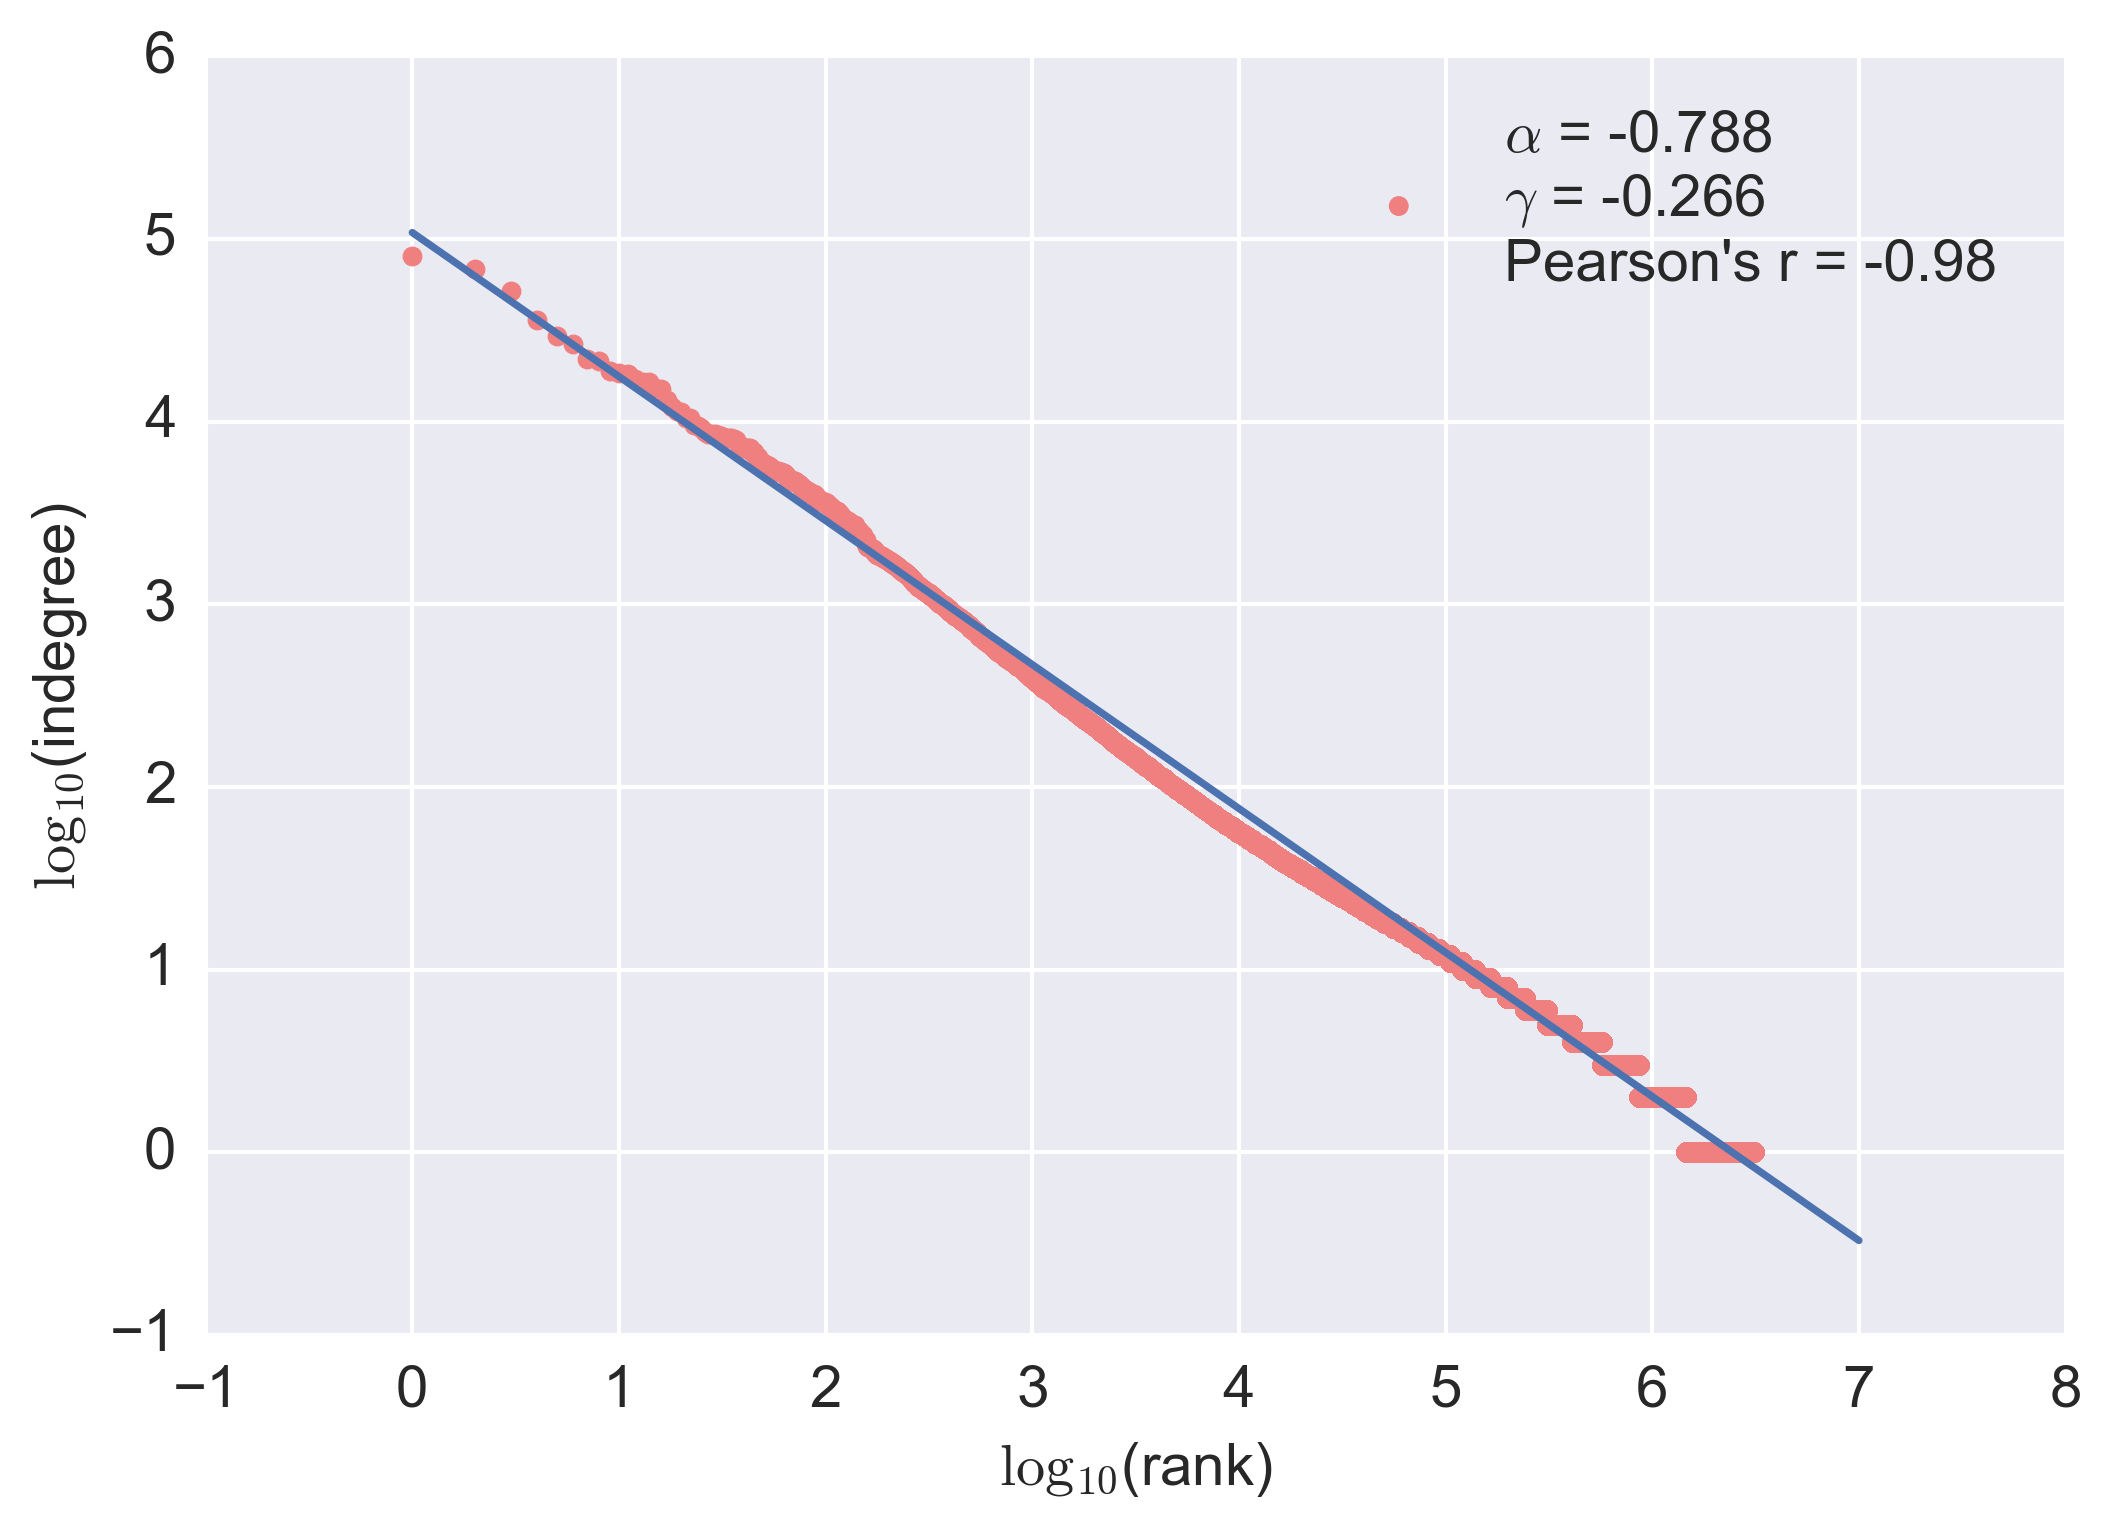
\includegraphics[width=\columnwidth]{graphics/ndegree_loglog.png}
  \caption{
    \textbf{FLN Degree Distribution}
  }
  We construct a log-log plot fit our results to a linear model. The result is a 
  an excellent fit with r = -0.98, yielding a power law exponent of -0.79. 
  The distribution appears scale free with most articles having fewer than 9 
  direct first links, while few hold most.
  \label{fig:degree distribution}

\end{figure*}
As a distribution, we examine the degree of the articles in the FLN with at least
one direct first link. The average n-degree 
is 3.6 direct links with a standard deviation of 89.5 links.
Only 4826 articles have more than 100 direct first links, $75\%$ have fewer than 
9. Overall the n-degree appears scale-free with an r value of -0.98 as a linear log-log fit and a power law exponent of -0.79. 



\subsection{Traversal Funnels}

Measuring only traversal visits and n-degree is limiting as it does not distinguish whether a particular article in a cycle 
is a funnel, directing many more paths inside the cycle than others. 
To distinguish among articles in a cycle, we also measured traversal funnels, or the number of 
paths an article directs towards a cycle. Here we count the number of traversal visits up to a cycle, 
so that accumulation does not flow to all articles in a cycle.
The importance here is to distinguish an article that happens to be connected to another article with many traversal visits 
from an article directly funneling many paths.

Measuring traversal funnels reveals a dramatically different structure where "Philosophy" stands unmatched by orders of magnitude:
\begin{figure*}[tp!]
  \centering	
  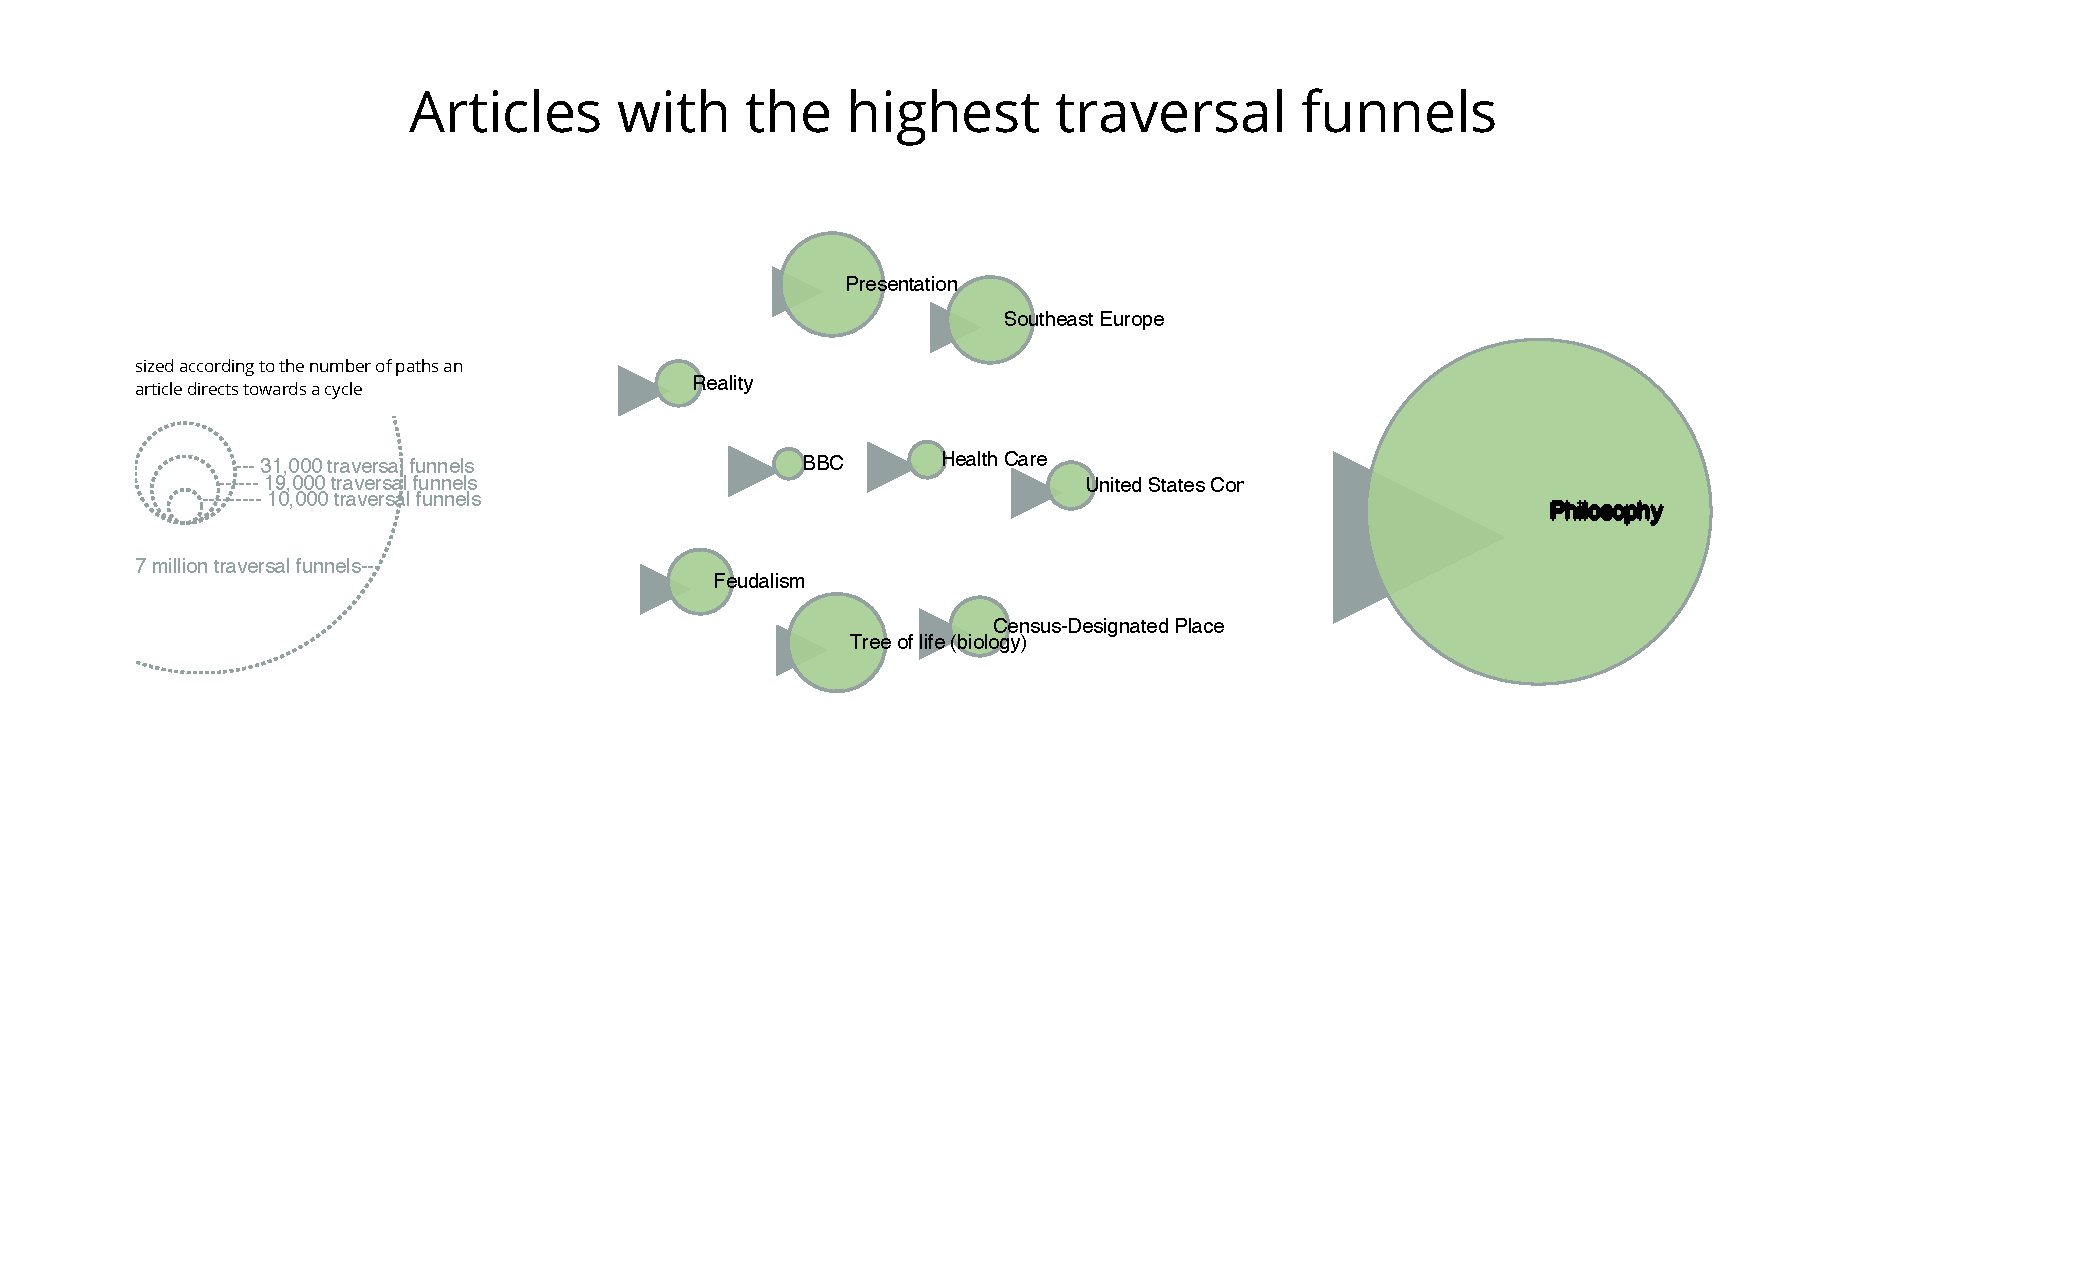
\includegraphics[width=\textwidth]{graphics/funnels.pdf}
  \caption{
    \textbf{Funnels}
  }
  \label{fig:Funnels}
\end{figure*}

Philosophy is not only a stand out the number of traversal visits, but also by the number articles "Philosophy" funnels into
its cycle. Of any article, the number of traversal funnels Philosophy holds exceeds 
all others by at least two orders of magnitude.
Next to the contribution of the largest funnels, "Philosophy" is a singularity. 
In proportion, "Presentation" holds only $0.4\%$ next to the number of traversal feeds for "Philosophy".
The second contributor to the Philosophy cycle is "Reality", funneling in a mere $0.2\%$ of traversals visits in the cycle.
Nevertheless, the other high ranking funnels are remarkably topical, culturally and politically important ideas.  For example, "Health Care", a recently high-contested legislative topic appears high on the list---Google trends indicates an uncharacteristic spike in search frequency between August-2009 and February-2010.
Other high ranking articles include key historical events such as the "Cold War" or critical scarce resource with recent 
media discussion such as "Fossil Fuel".
This coincidence of recent relevance and traversal feed rank suggests the First Link Network measurably represents
meaningful relationships not only among ideas, but also to English-speaking society. 

\red{TODO: add two regimes for power-law distribution}

\subsection{Article Popularity}

Using a recently released api, we compare the popularity of a page to our 
findings about the FLN. We measure popularity as the total number 
of page views in the english edition of Wikipedia in the month of 
October 2015 (the earliest full month for which the data is available). 
We find \dots

%========================Conclusion====================================

\section{Reflections}

The findings here should only be considered within the limitations of their context.
We examined only the English version of Wikipedia at a particular moment in time.
Furthermore, we only studied the First Link in the main body  of each article
as a means to related one article to another. Finally, Wikipedia, while the largest 
collection of human knowledge, is rife with the biases of the many contributing editors ((cite))
. Nevertheless, the findings do reveal
generalizable relationships, point to foundational notions, and uncover many curiosities.


Among the curiosities is the multiple appearance of scale-free distributions within the network. 
The three metrics we developed: path length, traversal visits, and traversal funnels are all marked 
by scale-free distributions. Few articles have most traversal visits, few paths have an exceptionally long path length, and even fewer
articles are responsible for funneling most paths. When measured against the traversal funnels, 
"Philosophy" emerges as an exceptional article by orders of magnitude. 
Nevertheless, many other foundational ideas emerged naturally within the First Link Network. 
Basins around "Community", "State", and "Science" reveal a foundational structure within the network. 
More curious is the emergence of recently prominent political and economics topics such as "Fossil Fuel" and "Health Care" 
within the highest ranking funnels. 
Wikipedia seems to reflect not only timeless foundations, but also the topical (at least within English speaking society).

Future work could examine other language versions of Wikipedia for potentially telling cultural or regional differences as well as expand the network to more than the First Link.
These findings also form the basis for the creation of a taxonomy where 
every idea, event, or object sits within a hierarchy of connected notions.
The taxonomy would extend a traditional word thesaurus beyond mere synonyms to a related hierarchy of concepts.
Applications could range from an enhanced thesaurus of ideas to psychological insights into how humans form associations.
Specifically, an ever-evolving reference of related hierarchical concepts can be applied to search engine algorithms 
or natural language processing.


\acknowledgments
Thank you to my friend RJ for pointing out the xkcd comic describing how the majority of links lead to "Philosophy," inspiring this research.


\newpage

\section{Appendix}

\subsection{Constructing The First Link Network}

To map Wikipedia's First Link Network, we use the freely-available XML dump of the English edition of Wikipedia. 
Rather than rely on a sample of articles from which to generalize, we opted to process the entirety of Wikipedia, 
eliminating any statistical error due to sampling.
We analyze the snapshot provided on November 2014, representing the state of Wikipedia at the time.
The November raw dump consists of 11 million articles: 4.7 million unique articles along with redirects
and disambiguations.
Knowing Wikipedia is an ever-evolving project with 10 edits every second and 750 new articles per day on average
((cite)), our aim is to characterize the dynamics of the First Link Network, not record a particular link between one
article and another.

Wikipedia renders and stores articles in MediaWiki markup, a markup language with syntax and keywords to format and mark elements in a page. Along with special syntax for links, MediaWiki markup includes templates for audio files, images, and side-bar
information.
While a human could accurately identify the First Link, to map the entire First Link Network of 11 million articles, we needed to programmatically untangled the body text from side-bar, header box, and invalid link elements.

While some libraries exist for MediaWiki Markup,
Approaches using existing libraries led to several bugs 
including trouble with nested links, nested parenthesis, unclosed tags, escape characters 
as well as compatibility with other libraries used to parse the XML.
Consequently,  we developed an algorithm for parsing the First Link in the XML version of each article.
Our parsing algorithm aimed to: 
1) accurately identify the First Link among other page elements, and 
2) efficiently do so---that is without needing for several passes through the data.
To process an article in a single pass, we developed a hierarchical system of flags:

\begin{figure*}[tp!]
  \centering	
  \includegraphics[width=\columnwidth]{graphics/flags.pdf}  
  \caption{
    \textbf{Parsing Algorithm of Wikipedia's XML dump}
     The highest flag in the hierarchy indicates a Wikimedia template used to mark an element in the side bar, display an image, link to an external file, or another Wikimedia project outside of Wikipeida. Next, to catch any remaining elements outside the main body we have a second flag for <ref>, <div> elements. Finally, we identify parenthesis to ensure we do not capture a link to a pronunciation key.
  }
  \label{fig:parsing algorithm}
\end{figure*}

The algorithm loops in three-character chunks to account for potentially nested elements, 
shifting by one character steps through the article markup.
If any markup triggers for a flag are detected, a flag is raised. 
Once a flag is raised, we stop processing and proceed to the next character
until the flag's closing markup.
A First Link is identified only if Flags 1, 2, and 3 are all off.
In this case, the entire link is retrieved. 
We then confirm the link is valid by filtering for MediaWiki keywords indicating external page or other projects
as well as common file extensions for 
((cite))
images, audio files, and the like.
The First Link of an article is then the earliest valid link with unraised flags.

To process the entirety of Wikipedia, we distributed the parsing and processing of the XML dump
across 112 cores of the UVM supercomputer cluster
\cite{vacc}
We then joined the results to form a hash table containing every Wikipedia article and its corresponding
First Link. The resulting network map is the basis of our analysis.


\subsection{Supplementary Tables}

\begin{figure*}[tp!]
  \centering	
  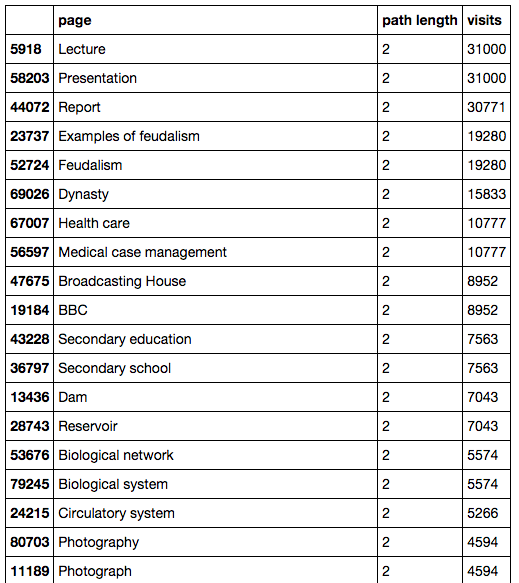
\includegraphics[width=\columnwidth]{graphics/top_2loops.png}
  \caption{
    \textbf{highest ranking 2-Cycles}
  }
  \label{fig:Highest Ranking 2-Cyles}
\end{figure*}

\begin{figure*}[tp!]
  \centering	
  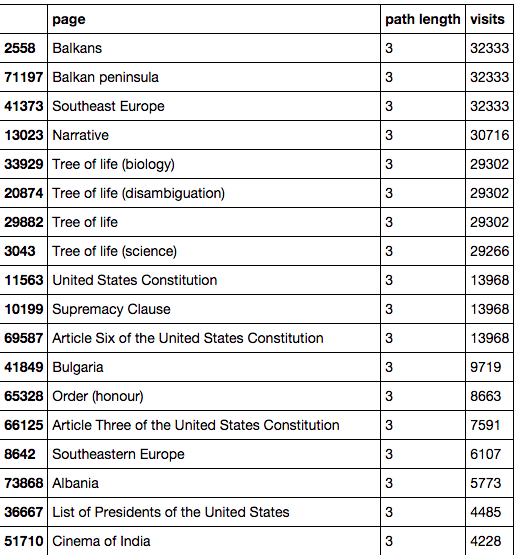
\includegraphics[width=\columnwidth]{graphics/top_3loops.png}
  \caption{
    \textbf{highest ranking 3-Cycles}
  }
  \label{fig:Highest Ranking 3-Cyles}
\end{figure*}

\begin{figure*}[tp!]
  \centering	
  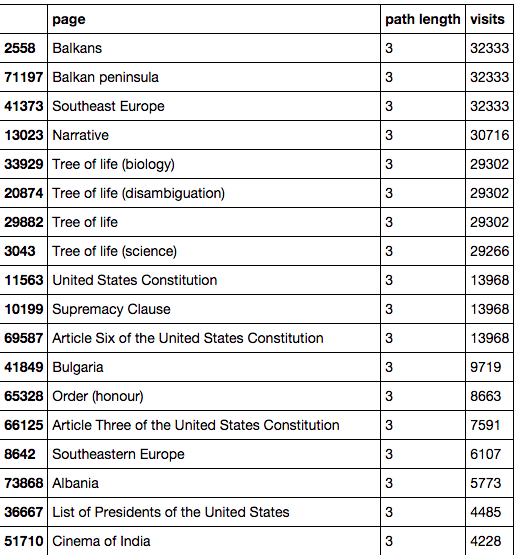
\includegraphics[width=\columnwidth]{graphics/top_3loops.png}
  \caption{
    \textbf{highest ranking 3-Cycles}
  }
  \label{fig:Highest Ranking 3-Cyles}
\end{figure*}

\begin{figure*}[tp!]
  \centering	
  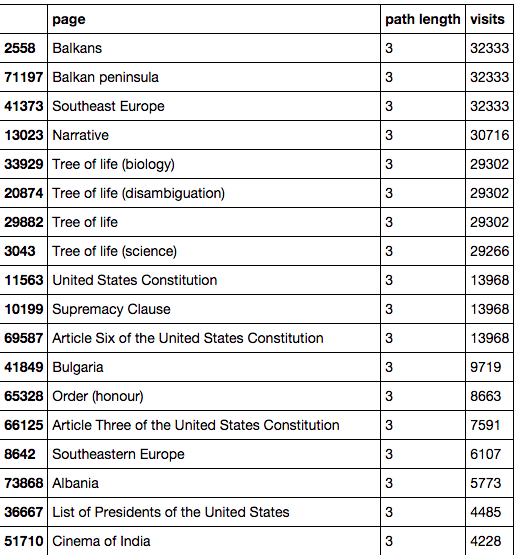
\includegraphics[width=\columnwidth]{graphics/top_3loops.png}
  \caption{
    \textbf{highest ranking 3-Cycles}
  }
  \label{fig:Highest Ranking 3-Cyles}
\end{figure*}

\begin{figure*}[tp!]
  \centering	
  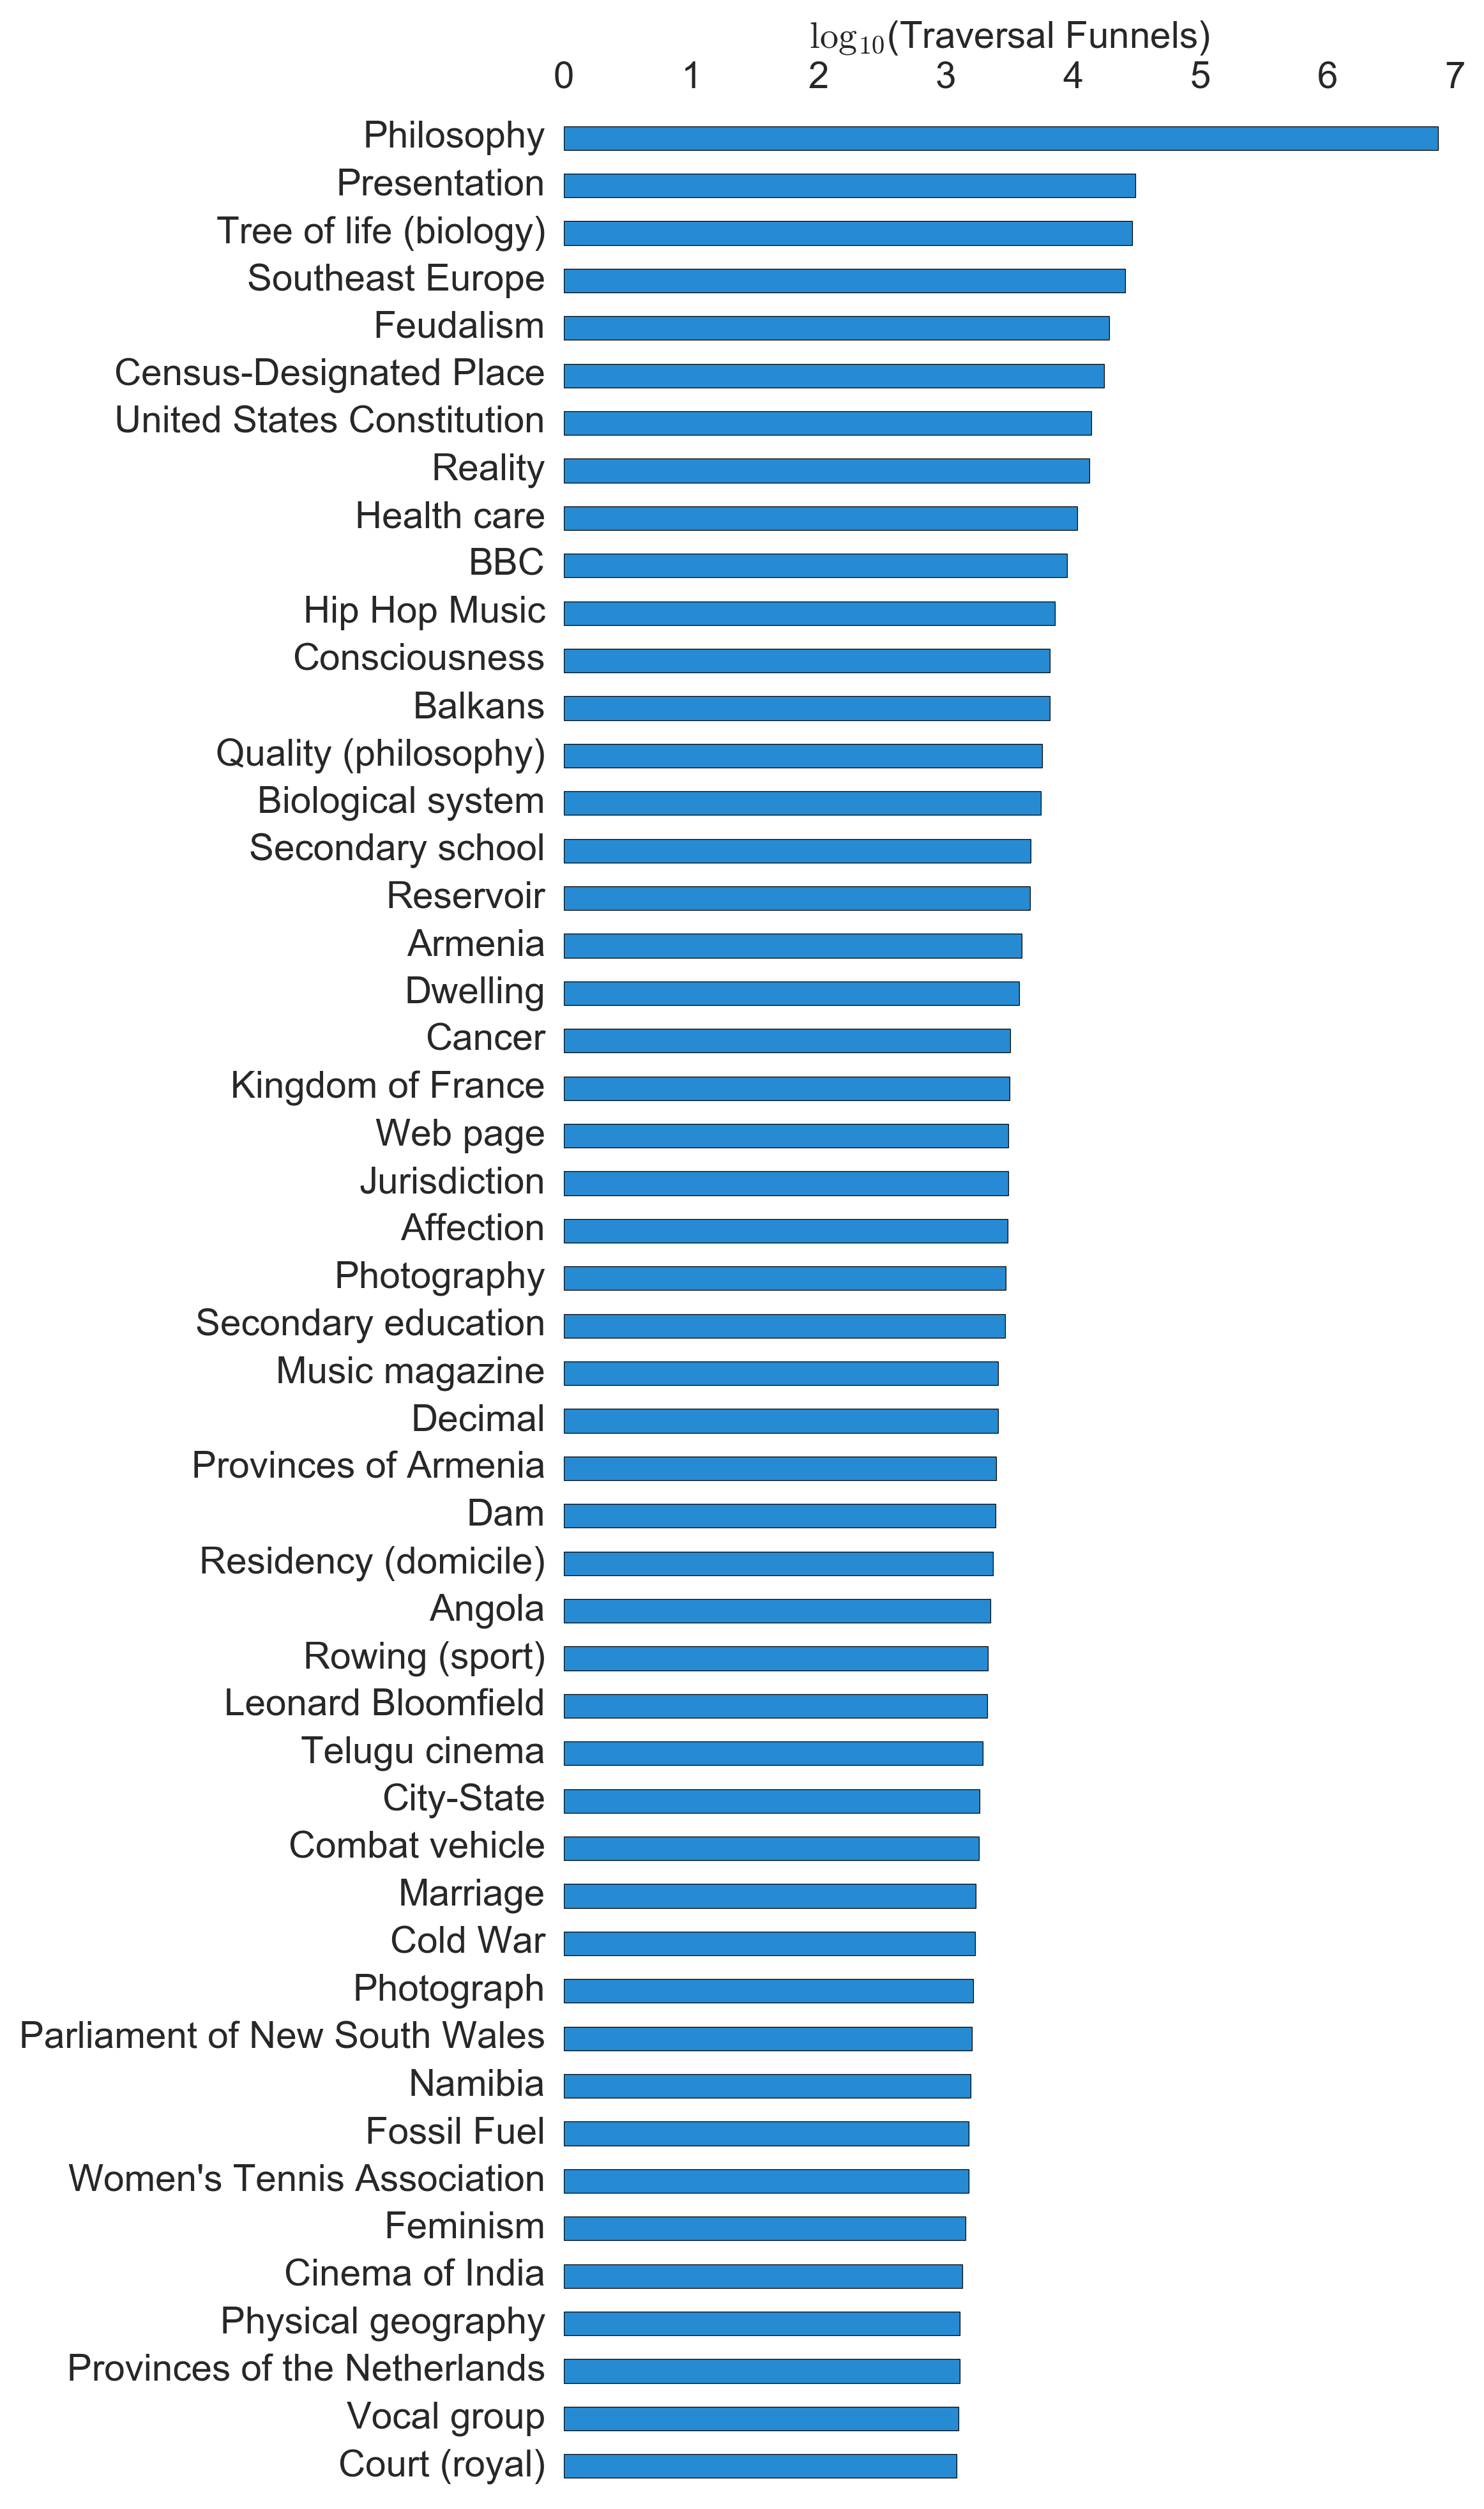
\includegraphics[width=\columnwidth]{graphics/top_funnels.png}
  \caption{
    \textbf{Highest Ranking Articles by Traversal Funnels}
  }
  \label{fig:Highest Ranking by Traversal Funnels}
\end{figure*}


\begin{thebibliography}{1}

      \bibitem{editors} Iba, Takashi, et al. "Analyzing the creative editing behavior of Wikipedia editors: Through dynamic social network analysis." Procedia-Social and Behavioral Sciences 2.4 (2010): 6441-6456.

      \bibitem{accuracy1} Holman Rector, Lucy. "Comparison of Wikipedia and other encyclopedias for accuracy, breadth, and depth in historical articles." Reference services review 36.1 (2008): 7-22.

      \bibitem{accuracy2} Giles, Jim. "Internet encyclopaedias go head to head." Nature 438.7070 (2005): 900-901.

       \bibitem{coverage} Halavais, Alexander, and Derek Lackaff. "An analysis of topical coverage of Wikipedia." Journal of Computer‐Mediated Communication 13.2 (2008): 429-440.

        \bibitem{bias_women} Hill, Benjamin Mako, and Aaron Shaw. "The Wikipedia gender gap revisited: characterizing survey response bias with propensity score estimation." PloS one 8.6 (2013): e65782.

      \bibitem{missing_entries} Williams, Jake Ryland, Clark, Eric M., Bagrow, James P., Danforth, Christopher M. \& Dodds, Peter Sheridan (2015). Identifying missing dictionary entries with frequency-conserving context models. Phys. Rev. E, 92, 042808.

      \bibitem{clustering} Banerjee, Somnath, Krishnan Ramanathan, and Ajay Gupta. "Clustering short texts using wikipedia." Proceedings of the 30th annual international ACM SIGIR conference on Research and development in information retrieval. ACM, 2007.

      \bibitem{semantic_relatedness} Gabrilovich, Evgeniy, and Shaul Markovitch. "Computing Semantic Relatedness Using Wikipedia-based Explicit Semantic Analysis." IJCAI. Vol. 7. 2007.

      \bibitem{disambiguating} Cucerzan, Silviu. "Large-Scale Named Entity Disambiguation Based on Wikipedia Data." EMNLP-CoNLL. Vol. 7. 2007.

      \bibitem{drugs} Clauson, Kevin A., et al. "Scope, completeness, and accuracy of drug information in Wikipedia." Annals of Pharmacotherapy 42.12 (2008): 1814-1821.

      \bibitem{stats} Wikipedia contributors. "Wikipedia:Statistics." Wikipedia, The Free Encyclopedia. Wikipedia, The Free Encyclopedia, 9 Nov. 2015. Web. 13 Nov. 2015.

      \bibitem{pagerank} Page, Lawrence, et al. "The PageRank citation ranking: bringing order to the Web." (1999).

      \bibitem{classifier} Chakrabarti, Soumen, Mukul Joshi, and Vivek Tawde. "Enhanced topic distillation using text, markup tags, and hyperlinks." Proceedings of the 24th annual international ACM SIGIR conference on Research and development in information retrieval. ACM, 2001.

      \bibitem{relevance} Kamps, Jaap, and Marijn Koolen. "Is Wikipedia link structure different?." Proceedings of the second ACM international conference on Web search and data mining. ACM, 2009.

    \bibitem{locke} Bolton, Martha Brandt. "The Taxonomy of Ideas in Locke’s {\it Essay} ", The Cambridge Companion to Locke's 'Essay Concerning Human Understanding'. Ed.Lex Newman.. 1st ed. Cambridge: Cambridge University Press, 2007. 67-100. Cambridge Companions Online. Web. 13 November 2015. http://dx.doi.org/10.1017/CCOL0521834333.004.

    \bibitem{aristotle} Studtmann, Paul, "Aristotle's Categories", The Stanford Encyclopedia of Philosophy (Summer 2014 Edition), Edward N. Zalta (ed.), \url{http://plato.stanford.edu/archives/sum2014/entries/aristotle-categories/}

    \bibitem{descartes} Smith, Kurt, "Descartes' Theory of Ideas", The Stanford Encyclopedia of Philosophy (Spring 2014 Edition), Edward N. Zalta (ed.), \url{http://plato.stanford.edu/archives/spr2014/entries/descartes-ideas/}


    \bibitem{hist_thesaurus} What is the Historical Thesaurus of the OED - Oxford English Dictionary (Oxford English Dictionary)
    http://public.oed.com/historical-thesaurus-of-the-oed/what-is-the-historical-thesaurus-of-the-oed/

    \bibitem{vacc} The authors acknowledge the Vermont Advanced Computing Core which is supported by NASA (NNX 06AC88G), at the University of Vermont for providing High Performance Computing resources that have contributed to the research results reported within this paper.
    \url{http://www.uvm.edu/vacc}

    \bibitem{wiki_views} Page Views for Wikipedia, Non-mobile site, Normalized (Page Views for Wikipedia, Non-mobile site, Normalized)
    \url{https://stats.wikimedia.org/EN/TablesPageViewsMonthly.htm}
\end{thebibliography}


\end{document}
